\documentclass{uofsthesis-cs}
\usepackage[noblocks]{authblk}
\usepackage{graphicx}
\usepackage{caption}
\usepackage{subcaption}
\usepackage{titlesec}
\usepackage{indentfirst}
\usepackage{hyperref}
\usepackage{booktabs}
\usepackage{makecell}
\usepackage{arydshln}
\usepackage{tikz}
\usepackage{algpseudocode}
\usepackage{algorithm}
\usepackage{textcomp}

\def\checkmark{\tikz\fill[scale=0.4](0,.35) -- (.25,0) -- (1,.7) -- (.25,.15) -- cycle;}

\title{Comparative analysis of Gene Finding tools when applied to
  \textit{Trichoderma} genomes} %\author{Connor Burbridge} \affil{USask
  %NSID: cbe453 \\ USask ID no.\ 11162928 \\ Supervisors: Dave
  %Schneider \& Tony Kusalik\\}

\parindent=14pt

\abstract{placeholder}

\acknowledgements{I would like to acknowledge both
  Dr. Kusalik and Dave Schneider for their excellent support and
  mentorship during both COVID and my MSc. project. I would also like
  to thank Brendan Ashby and Dr. Leon Kochian for providing both data
  and additional financial support.}

\loa{
\abbrev{DNA}{Deoxyribonucleic acid}
\abbrev{RNA}{Ribonucleic acid}
\abbrev{CDS}{Coding sequence}
\abbrev{Mb}{Megabases}
\abbrev{Kb}{Kilobase}
\abbrev{WGS}{Whole Genome Shotgun (sequencing)}
\abbrev{NGS}{Next generation sequencing}
\abbrev{PCR}{Polymerase chain reaction}
\abbrev{GMO}{Genetically modified organism}
\abbrev{CPU}{Central processing unit}
\abbrev{GC}{Guanine cytosine}
\abbrev{HMM}{Hidden Markov model}
\abbrev{UTR}{Untranslated region}
\abbrev{GFF}{General feature format}
\abbrev{BUSCO}{Benchmarking Universal Single-Copy Orthologs}
\abbrev{RSMI}{Root, Soil and Microbial Interactions}
\abbrev{MITE}{Minature inverted-repeat transposable element}
\abbrev{TIR}{Terminal inverted repeat}
\abbrev{TDR}{Terminal direct repeat}
\abbrev{maybe}{Should I include tools like BLAST and resources like NCBI?}
}


% From Yujie: Assume I am only working on chapter 2 for now, so only include that
% chapter in the main document. This is useful for working on a single
% chapter at a time, and speeds up compilation.
\includeonly{chapter-2}


\begin{document}
\maketitle
\frontmatter


%\chapter{Introduction}
The study of organisms in Biology is a highly complex complex process
involving many disciplines. To better understand how these organisms
function, we must braker down the problem into different
sub-problems. One important sub-problem in biology is the
understanding of the molecular tools and processes used by cells to
function in normal and abnormal environmental scenarios or stress
conditions. These conditions may include disease and environmental
stress for example. However, previous work in biology has shown that
the underlying backbone of information, known as the genome, can vary
widely between different organisms in many aspects, such as overall
structure, length, ploidy, methylation, and overall gene content. All
of these aspects can affect the survival of an organism in any given
environment, some of which may be interesting to researchers. As an
example, one of the most popular and extensively studied diseases is
cancer. Through the study of human genomes, researchers identified a
key gene, named TP53, involved in the suppression of
tumours. Functional mutations affecting this gene can result in
increased risk of cancer. Understanding how and why TP53 suppresses
tumours can provide insight into future cancer prevention methods and
treatments. These genes can then be mapped to the genome of the
organism to identify its location.

This general workflow can be applied to features of interest from
organisms in all branches of life. To facilitate this process of
identifying genes from a genome, the process of genome annotation was
developed. In this case, instead of identifying a gene of interest and
then mapping it back to the genome, gene finders identify potential
genes from a reference genome before truly knowing their function or
if the candidate is truly untilized by the organisms. This set of
potential genes acts as a reference for future research. However, to
generate a reliable set of possibe genes, a gene finder must be
supplied with a suitable high quality genome. In many cases,
researchers may be studying a specific strain or variety of organism
that differs from the reference assembly and annotation available for
the organism of interest. Rather than using the reference assembly for
analysis, it may be beneficial to generate a new assembly for the
unique variety or strain, which must then be passed through a gene
finding tool. With the variety of gene finding tools and approaches,
the choice of an appropriate tool can affect the resulting gene
set. This problem raises a question. Do the results from gene finding
tools differ? And more importantly, how should one compare results
from gene finding tools when there is no reference annotation for a
specifc variety in question? Most genome annotation tools benchmark
their performance in comparison to an existing reference annotation,
which is usually considered to be of suitably high quality. This is
not possible in the case of unique assemblies, and so the devleopment
of a comparative methodology is in order.


\chapter{Background}
%\section{Genomics}
%Genomics is a wide area of study focusing on the genomes of organisms
%from all varieties of life. A genome is a sequence of characters that
%contains the fundamental set of `rules' used to create what we know as
%life. One can think of a genome as a set of instructions that our
%cells use in order to complete the tasks that make us function. A
%genome is comprised of tightly bundled sequences of DNA, which are
%stored in the nucleus of cells. These bundles of DNA contain sections
%known as genes, which can be thought of as the tools described by the
%set of instructions. These tools carry out a vast number of processes
%ranging from no known function at all to genes that are key in
%protecting against diseases cancer. Genomes can vary widely in size,
%ranging from small bacterial genomes of roughly 4 Mb up to
%approximately 149000 Mb. Piecing together genomes provides numerous
%opportunities to understand other `omics' within cells, such as
%proteomics, metabolomics, transcriptomics and epigenomics.

Chapter one provides a brief background on \textit{Trichoderma} and gene prediction tools, providing context for this research. Section~\ref{lit:evolution} discusses the evolutionary mechanisms that may have led to the increased production of secondary metabolites in \textit{Trichoderma} species, such as horizontal gene transfer, gene duplication, and transposable elements.Section~\ref{lit:novel-genomes} discusses the novel \textit{Trichoderma} genomes that were sequenced and assembled as part of this work, and how they relate to the research questions. Section~\ref{lit:similarity-searches} discusses the structure of eukaryotic genes how gene finders predict them, while section~\ref{lit:secondary-metabolites} provides an overview of secondary metabolites and their importance in \textit{Trichoderma} species. Finally, section~\ref{lit:comp-motiv} provides an overview of comparative studies of gene prediction tools in \textit{Trichoderma} species, and how this work aims to fill the gap in literature.

\section{\textit{Trichoderma} Species and their Features}
\label{lit:features}

\textit{Trichoderma} are a genus of ascomycete fungi found in a wide
variety of soils, and are well-known for their use in biomanufacturing
of cellulases and hemicellulases as well as their roles as non-toxic,
avirulent opportunistic plant symbionts~\cite{woo2023a}~\cite{kubicek2019a}. 
Many of these features \textit{Trichoderma}
can be attributed to the large number of secondary metabolites
produced by these fungi, which are used to interact with plants and other organisms in the soil~\cite{Mukherjee2012}. \textit{Trichoderma} species differ in the number of secondary metabolites they produce, with some species producing more than others~\cite{Mukherjee2012}. This variation in secondary metabolite production is of great interest to researchers, as it can provide insight into the evolutionary processes that have shaped \textit{Trichoderma} species over time.

There are many mechanisms organisms may leverage that result in gain or loss of gene function, and ultimately the evolution of a species. One well-studied mechanism is that of horizontal gene transfer (HGT), which is the process of acquiring genetic material from another organism, rather than through inheritance from a parent organism~\cite{goncalves2024}. HGT is a common mechanism in bacteria, but it has also been observed in fungi, including \textit{Trichoderma} species~\cite{goncalves2024}. Another mechanism of interest is the duplication of genes, which can result in the production of more than one copy of a gene, leading to increased expression of that gene~\cite{goncalves2024}. This is particularly relevant in the case of secondary metabolite production, as many \textit{Trichoderma} species have been shown to have multiple copies of genes involved in secondary metabolite production~\cite{Mukherjee2012}. Lastly, transoposable elements (TEs) are another mechanism of interest, as they can insert themselves into the genome and disrupt or enhance the expression of genes~\cite{goncalves2024}. TEs have been shown to play a role in the evolution of \textit{Trichoderma} species, particularly in the case of secondary metabolite production~\cite{goncalves2024}. 

Interestingly, both HGT and TEs tend to present themselves in regions where GC content differs from the rest of the genome, ~\cite{goncalves2024}. Abnormal GC content is also associated with other genomic features, such as centromeres~\cite{plohl2014a} and repetitive regions~\cite{winter2018}, both of which may have an effect on the production of secondary metabolites in \textit{Trichoderma} species. As a result, it is important to consider the GC content of a genome when studying \textit{Trichoderma} species, which forms the basis of the Research Question ~\ref{rq:anomalous-sequence-content}. Some studies have shown that \textit{Trichoderma} species contain very few if any transposable elements, which is unusual for fungi~\cite{kubicek2011}. It is hypothesized that TEs were lost in \textit{Trichoderma} due to repeat induced point mutations (RIP), which is a process that occurs in fungi where TEs are silenced and eventually lost from the genome~\cite{kubicek2011}. Genes responsible for RIP mutations also tend to target CA dinucleotides, converting them to TA nucleotides, which explains the low GC content observed in some regions of \textit{Trichoderma} genomes~\cite{goncalves2024}.

%One common theory for the increase in secondary metabolites is that \textit%{Trichoderma} initially evolved as a parasite or saprotroph of plants, due to their abundant production of cellulases and plant wall degrading enzymes~\cite{kubicek2019a}. In addition to saprotrophy, \textit{Trichoderma} species are also mycoparasitic, feeding on other Ascomycete and closely related fungal species~\cite{Druzhinina2018}. As a result, it is hypothesized that the elevated production of secondary metabolites in \textit{Trichoderma} arose from the constant change and competition for resources in the environments in which they evolved.~\cite{Mukherjee2012}. While many studies have been conducted on the mechanisms behind fungal evolutionary processes, the process of horizontal gene transfer (HGT), is of particular interest in the case of \textit{Trichoderma}~\cite{goncalves2024}.
Given the proximity of \textit{Trichoderma} species to other fungi, bacteria, and plants in soils, it is possible that \textit{Trichoderma} species acquired genes which are involved in response to antagonistic and sympathetic intercellular interactions from other organisms. While difficult to prove, studies have shown that HGT events have occurred in a number of fungal species~\cite{fitzpatrick2012}. It is also important to note that some \textit{Trichoderma} species have higher numbers of genes involved in secondary metabolite production than others, indicating an evolutionary divergence, making comparative analysis of \textit{Trichoderma} species and strains a useful tool for understanding the mechanisms behind secondary metabolite production~\cite{Mukherjee2012}.

\section{Evolutionary Landscape of \textit{Trichoderma}}
\label{lit:evolution}

The evolutionary landscape of \textit{Trichoderma} species is an important aspect of this work. DC1 and Tsth20 have not yet been classified into a specific \textit{Trichoderma} species, and further understanding of their evolutionary relationships to other \textit{Trichoderma} species may help explain how DC1 and Tsth20 originated. 
Figure~\ref{fig:phylogeny} shows the phylogenetic relationships among selected \textit{Trichoderma} species as well as the outgroup \textit{Fusarium graminearum}. The tree was constructed using cursory alignments of the Rpb2 gene, which is a commonly used gene for phylogenetic analysis in fungi~\cite{an2022}. Representative Rpb2 proteins from the various fungal species were extracted from the NCBI resource for fungal orthologs, while representative Rpb2 proteins from DC1 and Tsth20 were identified from the results generated later on in this work. \textit{Trichoderma} species separate into a number of distinct clades, and these clades can vary between studies as evidenced by the low confidence in placement of \textit{T. atroviride} and \textit{T. gamsii}. Lack of confidence in evolutionary relationships is not uncommon in \textit{Trichoderma} species, and is likely due to the high levels of horizontal gene transfer and gene duplication that have occurred in these species~\cite{goncalves2024}. This makes \textit{Trichoderma} species interesting to study but difficult to classify. 

\begin{figure}
    \centering
    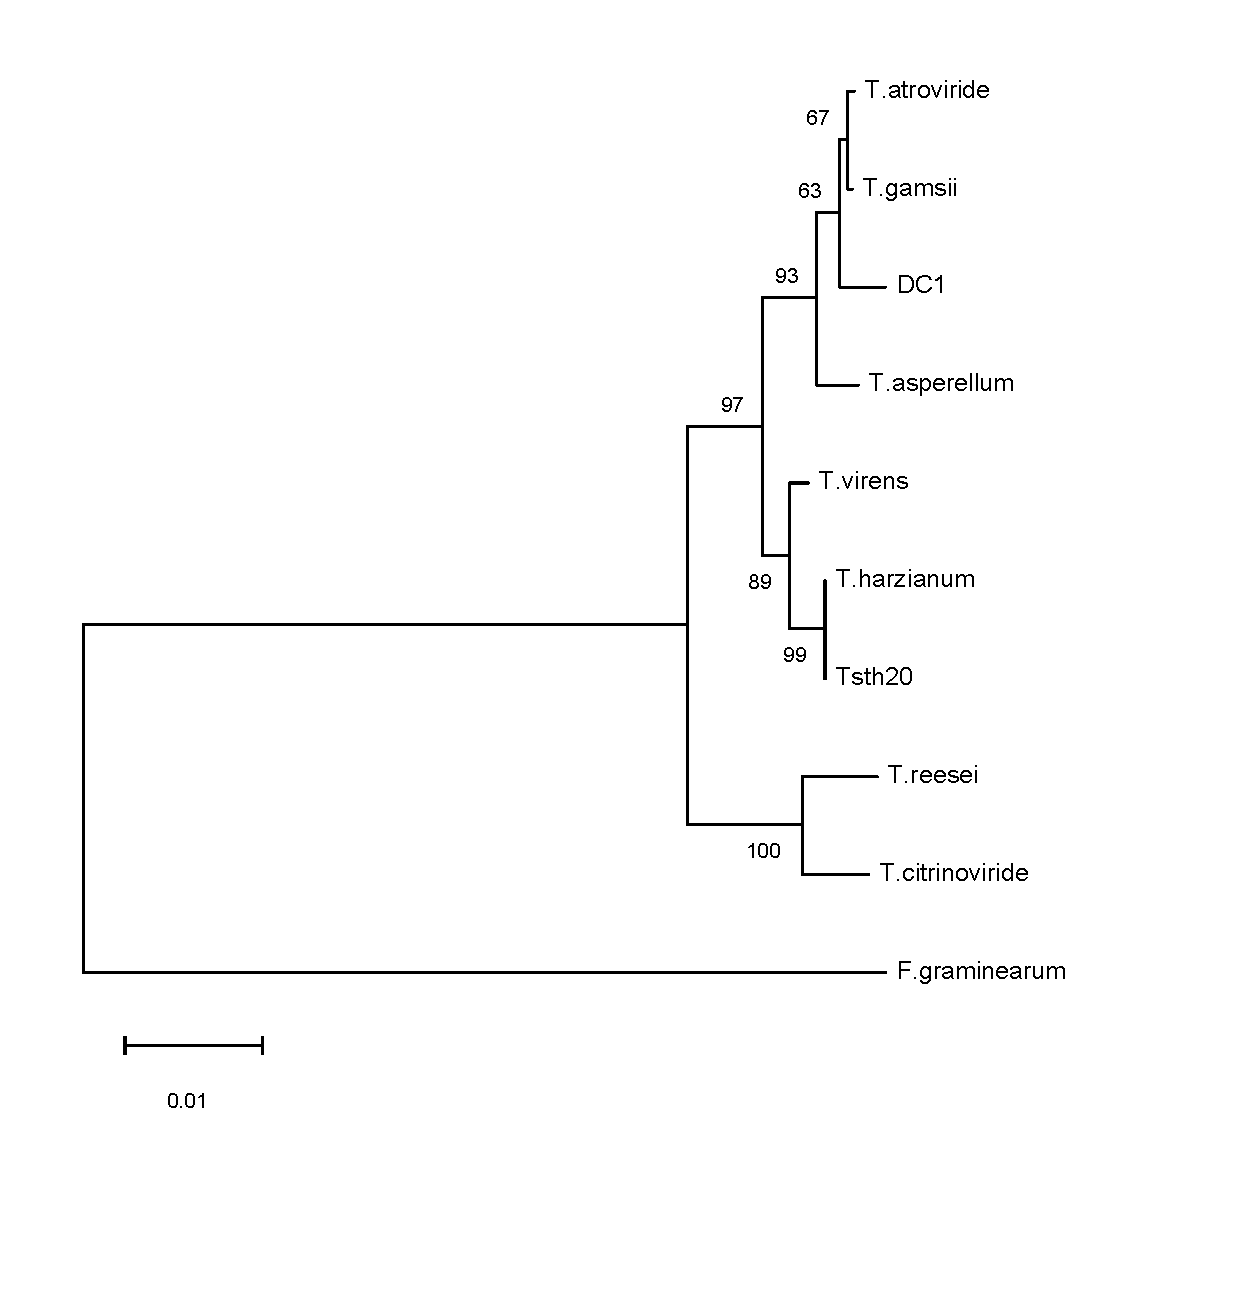
\includegraphics[width=\textwidth]{figures/trichoderma-phylogeny-few-outgroups.pdf}
    \caption{Phylogenetic tree illustrating relationships among selected \textit{Trichoderma} species based on multiple sequence alignments of Rpb2. Evolutionary history was inferred using the Neighbour-Joining method~\cite{Saitou1987}. The optimal tree with the sum of branch length = 0.146 is shown. The percentage of replicate trees in which the associated taxa clustered together in the bootstrap test (1000 replicates) are shown next to the branches~\cite{Felsenstein1985}. The tree is drawn to scale, with branch lengths in the same units as those of the evolutionary distances used to infer the phylogenetic tree.}
    \label{fig:phylogeny}
\end{figure}

Phylogeny is also important when selecting genomes for comparative analysis of bioinformatics tools. Some tools may vary in their performance depending on the nature of the genome they are applied to, making a heterogeneous selection of genomes important for understanding the performance of the tools in different contexts. In this work, we selected three well-studied \textit{Trichoderma} species, \textit{T. reesei, T. harzianum}, and \textit{T. virens} for future comparisons, which are all commonly used in research and industry, but are relatively distant from each other evolutionarily according to more detailed studies~\cite{an2022}. 

%\section{Environmental Stress}

%Crop resistance to environmental stressors is a necessity for crop
%health and overall crop yields. Current popular methods for crop
%protection involve the use of pesticides and genetically modified
%organisms, which can be expensive and potentially politically dividing
%in the case of GMOs~\cite{doi:10.1080/10408390600762696}. In addition,
%crops suffer when soils are not sufficient for crop growth and
%health. Soil insufficiencies can result in drought stress as well as
%nutrient stress, leading to poor overall yields.

\section{Novel \textit{Trichoderma} Genomes}
\label{lit:novel-genomes}
Recently, two strains of \textit{Trichoderma}
have been identified in the prairie regions of Alberta and
Saskatchewan. These two strains, named Tsth20 and DC1, have been found
to have beneficial properties when used as an inoculant for plants in
the soils. Tsth20 has been classified into the \textit{Trichoderma harzianum} group, and may act as a bioremediation tool in soils contaminated with hydrocarbon content. DC1, while not yet classified, is believed to confer salt and drought tolerance to plants in dry, salty soils. While, bioremediation and resistance to drought tolerance has been investigated in other strains of
\textit{Trichoderma}~\cite{senizza2023}, the study of new strains is still useful in the effort of discovering unique mechanisms used by \textit{Trichoderma}. Little is known about the mechanisms at work in these strains, so DC1 and Tsth20 were sequenced at the Global Institute for Food Security in an initial attempt to better understand the mechanisms at work in these genomes. While this research does not explicitly identify genomic elements related the beneficial properties of these genomes, it may serve as a foundation for future research of \textit{Trichoderma}. The assembly of these genomes come as a result of Research Question~\ref{rq:assembly-results}.

\section{Gene Predictions and Complementing Similarity Searches}
\label{lit:similarity-searches}
Gene prediction methods are generally based on the idea that genes can be
identified by searching for patterns in a sequence, which match an expected gene structure or model. These gene structures begin from a $5'$ start codon, continue through a series of exons and introns, and end with a $3'$ stop codon~\cite{loftus2003a}. Flanking the gene structure are promoter regions, which are typically found upstream of the start codon, and untranslated regions (UTRs), which are found both upstream of the $5'$ start codon and downstream of the $3'$ stop codon. Promoter regions are important for the regulation of gene expression, while UTRs are important for the stability and translation of the mRNA transcribed by the gene~\cite{loftus2003a}. Sequences are translated from the $5'$ start codon through to the $3'$ stop codon, splicing together exons and ignoring introns. An example of a eukaryotic gene structure is shown in Figure~\ref{fig:gene-structure}.

\begin{figure}[ht]
    \centering
    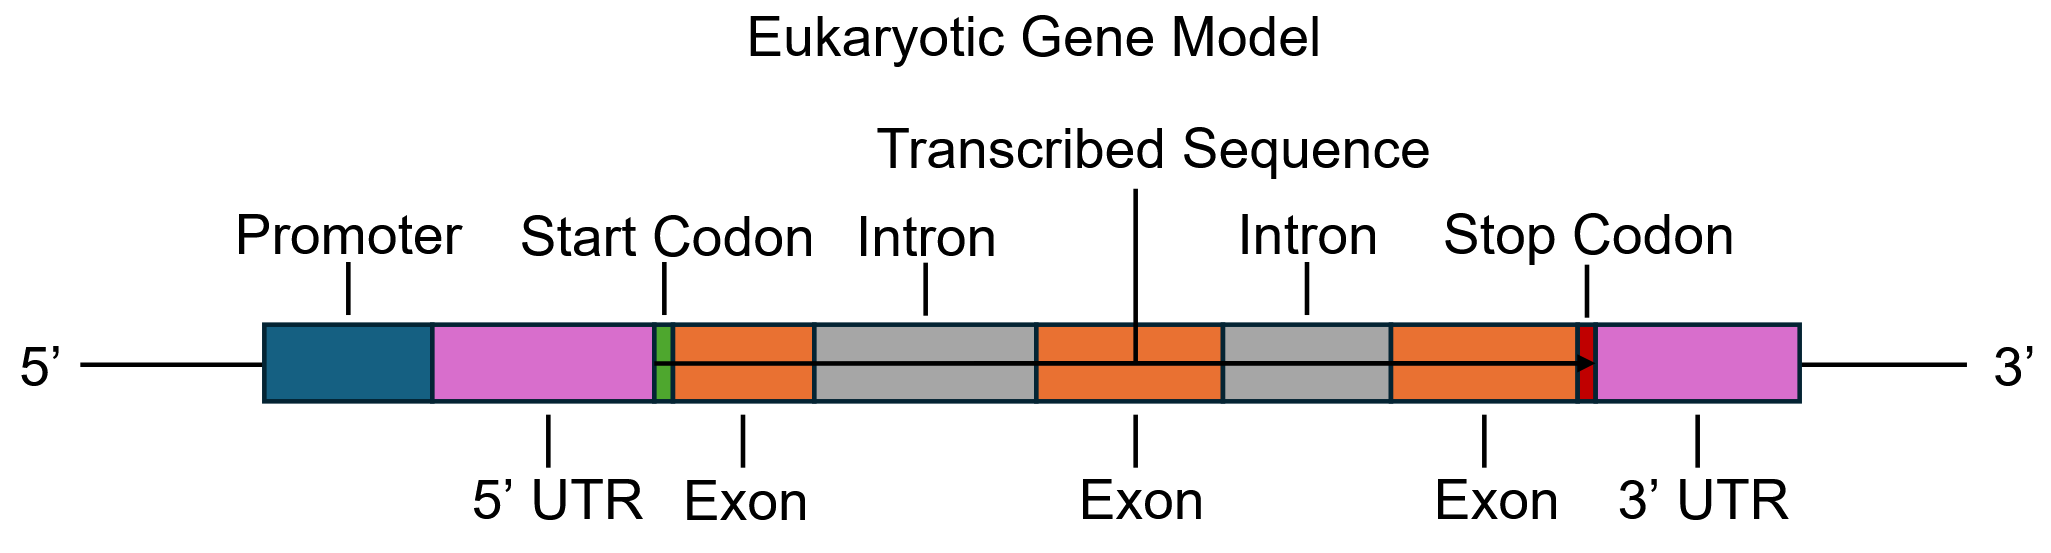
\includegraphics[width=0.8\textwidth]{figures/gene-model-fig-msc.png}
    \caption{Example of a eukaryotic gene structure, showing a promoter region (blue), the $5'$ and $3'$ UTRs (purple), start codon (green), exons (orange), and introns (grey). The evrected arrow indicates the direction of transcription. }
    \label{fig:gene-structure}
\end{figure}

Gene prediction methods vary in their approach, but they generally fall into two categories: \textit{ab initio} methods and evidence-based methods~\cite{ejigu2020a}. \textit{Ab initio} methods rely on the identification of patterns in the sequence that match an expected gene structure, while evidence-based methods use prior information such as RNAseq data, expressed sequence tags (ESTs), and expressed protein sequences to identify genes within a new genome~\cite{ejigu2020a}. Gene prediction methods can also vary in their ability to identify different components of a gene, such as the promoter region, UTRs, and introns. Some methods may only identify the coding sequence (CDS) of a gene, while others may also identify the promoter region and UTRs~\cite{ejigu2020a}. Making things more complicated, different gene prediction tools may predict different combinations of exons and introns for a gene, and some tools may even predict multiple combinations of exons and introns, leading to multiple transcripts for the same gene. As a result, different transcripts may produce different proteins, or the same protein with different post-translational modifications, which can significantly impact the function of the resulting protein~\cite{ejigu2020a}. Given the already complex nature of secondary metabolites, it is important to consider the impact of variability in gene prediction methods, especially in the case of \textit{Trichoderma} species and their secondary metabolite production. This consideration is one of the main motivators behind this research, and forms the basis of Research Question~\ref{identify-regions}.

Many gene prediction tools have been developed over the years, each with its own strengths and weaknesses. Some tools are designed to be fast and efficient, while others are designed to be more accurate and comprehensive~\cite{ejigu2020a}. As mentioned earlier, gene finding tools generally fall into one of two categories: \textit{ab initio} and evidence-based. \textit{Ab initio} methods are often used when no prior information is available, while evidence-based methods are used when prior information is available~\cite{ejigu2020a}. 

While the basic structure of a gene may be present in a sequence, that does not mean that the gene codes for a functional protein, or in the case of secondary metabolites, a component that helps produce them. To assess potential function of a gene product, gene prediction methods are often used in conjunction with similarity searches, which compare the predicted genes to known genes in other organisms to identify potential functions, and serve as a form of validation for the predicted genes~\cite{loftus2003a}. 
Similarity searches can come in several different forms, such as blast searches, which compare the predicted genes to a database of known proteins, or InterProScan, which compares the predicted genes to a database of known protein domains and binding motifs~\cite{loftus2003a}. These similarity searches can provide additional information about the predicted genes, such as potential functions, and can also help to validate the predicted genes by comparing them to known genes in other organisms. Similarity searches can also be used to evaluate the completeness of the predicted genes. One example would be comparing predicted genes to a set of conserved single-copy orthologs expected in fungal genomes, such as those provided by BUSCO~\cite{manni2021a}. Together, these methods can provide a more complete picture of the gene predictions and their potential functions, and can help to identify potential targets for further research. This forms the basis of Research Questions~\ref{rq:interproscan},~\ref{rq:tblastn}, and~\ref{rq:busco-completeness}.

\section{Secondary Metabolites}
\label{lit:secondary-metabolites}

While cellular products essential to an organism's viability are
of great interest, there are a vast number of cellular products that while not
essential, still provide great benefit to the
organism and may be necessary for survival in some situations~\cite{Craney2013}~\cite{Mukherjee2012}. These other cellular products are known
 as secondary metabolites, and they are involved in several roles ranging 
 from cellular signalling to antibiotic activity, making them a frequent 
 subject of study in pharmaceutical research. Enzymes that produce 
 secondary metabolites are comprised of non-ribosomal peptide synthetases 
 (NRPS) and polyketide synthetases (PKS), which synthesize amino acids and 
 other basic enzymatic building blocks into proteins~\cite{komaki2020}. 
 Genes encoding the NRPSs and PKSs responsible for production of secondary 
 metabolites are often found in clusters within a genome, but their 
 products remain unknown~\cite{Mukherjee2012}. 
 
 The evudy of these products is difficult, as the genes encoding the modules that make up NRPSs and PKSs are not expressed under normal laboratory conditions~\cite{Mukherjee2012}. The evPSs and PKSs that have been studied
 have been shown to be large enzymatic structures containing several 
 functional modules, each responsible for a specific step in the synthesis 
 of a protein~\cite{Mukherjee2012}. Studying these complicated mechanisms and their genes requires as close to a complete set of gene predictions as possible, as the absence of one gene encoding a module could affect the entire protein complex. This concept of completeness of gene predictions is explored in Research Question~\ref{rq:busco-completeness}. 
 In addition, gene predictions can be processed further with tools such as antiSMASH, which can identify secondary metabolite biosynthetic gene clusters (BGCs) in a genome~\cite{blin2023}. Comparison of predicted genes with known secondary metabolite BGCs can provide insight into completeness of the predicted genes with a specific focus on secondary metabolite production. This work is not covered in this thesis, but is worth noting for context as it is a common approach in the field of secondary metabolite research.

 Another interesting feature of NRPSs and PKSs is the length of the genes encoding them, which can be quite long, often exceeding 10,000 base pairs in length~\cite{komaki2020}. Examining the outputs of gene prediction tools can provide insight into the lengths of predicted genes, and whether or not the tools are able to capture the full length of these large genes. This topic serves as the basis for Research Question~\ref{rq:gene-lengths}.  

 %Given the modular nature of NRPSs and PKSs, one can assume that many genes %are responsible for the production of secondary metabolites. Thus, it is %important that methods used for the identification of genes involved in %secondary metabolite production are able to identify as many of those genes %as possible. Failure to identify these genes may result in an incomplete %understanding of the secondary metabolite production process, and may also %result in the loss of potential targets for further research. With this in %mind, it is important to consider the methods used for identification of %genes in a genome, as the methods used can have a significant impact on the %results, forming the basis of Research Questions ~\ref{rq:number-of-features} %and ~\ref{rq:gene-lengths}. 

\section{Gene Prediction Tools in Fungi}
\label{lit:comp-motiv}
With the biological context laid out, we can now turn our attention to the computational aspect of this work. Many \textit{Trichoderma} species have been assembled and annotated in the past, mostly for the purpose of understanding the mechanisms behind secondary metabolite production~\cite{Mukherjee2012}. Gene predictions in this context are typically compared against sequences from other organisms to derive functional information, and to validate the predicted genes~\cite{loftus2003a}. In contrast, very few studies have been conducted comparing gene prediction tools in fungal genomes, and even fewer have been conducted in \textit{Trichoderma} species. This is surprising, given the large number of gene prediction tools available, and the fact that many of them are used in the field of fungal genomics~\cite{ejigu2020a}. Comparisons of gene prediction tools are common when new tools are released, but these comparisons are often limited to a small number of tools, and tend to be focused on achieving higher counts of interesting genes, rather than comparing the results in a biological context~\cite{min2017}. Complicating the matter further, the quality of genome sequences available may vary, making evaluation of different gene prediction tools difficult when working with multiple genomes and lesser-studied fungal species with low quality assemblies. Given the gap in literature regarding comparative analysis of gene prediction tools in \textit{Trichoderma} species, and the availability of the novel DC1 and Tsth20 genomes, this work aims to fill that gap by comparing the outputs of several gene prediction tools on these two genomes along with three other frequently studied \textit{Tichoderma} species.

%\section{Genome Assembly}

%Sequence assembly has been a long-standing problem in the field of
%bioinformatics~\cite{nagarajan2013a}. Determining the correct order and
%combination of smaller subsequences into an accurate complete sequence
%assembly is computationally difficult in terms of compute resources
%such as memory, CPU cycles and storage required for input
%sequences~\cite{nagarajan2013a}. In addition to these difficulties,
%there can be other issues encountered during assembly due to the
%nature of the data or genomes themselves, such as low quality base
%calls for long read data, which is not necessarily the case today, or
%the inherent content of genomes themselves using repetitive regions as
%an example. Insufficient data may result in short, fragmented
%assemblies, depending on the size of the genomes, while sequence data
%that is not long enough can fail to fully capture repetitive regions
%in an assembly. A wide range of assembly tools have been developed
%with their own unique approaches to the genome assembly problem, so it
%is important to use an appropriate assembler for the task at hand, and
%also important to evaluate the assembly thoroughly.

%Genome assembly tools generally approach the assembly problem using a
%graph-based approach. The evst common graph-based approach is the de
%Bruijn graph assembly~\cite{compeau2011a}. A graph in this context, is
%set of nodes (\textit{k}-mers from sequences) connected by edges
%(overlaps between \textit{k}-mers). Traversing through this graph
%results in longer subsequences that ultimately result in a set of
%sequences referred to as an assembly. In the early years of long read
%sequence data, sequencing platforms encountered difficulties producing
%consistently high scores for base calls when sequencing. To combat
%this, some assembly workflows may also include a polishing or
%correction step once the initial assembly is completed in which high
%quality short read sequences are used as supplemental information to
%correct low quality regions in the assembly. These low quality base
%calls are typically not present in modern long read sequencing
%approaches as the methodology and quality of calls have improved
%drastically. While the polishing step is arguably unnecessary in
%modern assemblies, the polishing programs remain available should
%researchers be interested in applying additional reads for polishing.

%One approach to aid in the previously mentioned issue of assembly
%correctness is to use a combination of long and short reads in what is
%known as a hybrid assembly. Combining both highly accurate short reads
%with deep coverage along with less accurate but much longer reads can
%produce high quality genome assemblies that capture long repetitive
%regions. Hybrid assembly approaches have been shown to produce high
%quality assemblies in a wide variety of organisms as the combine long
%read data with short data to produce assemblies that properly
%represent long repetetive regions with additionaly high quality
%Illumina sequences for correction. Once assembled, the sequences must
%also be evaluated with measures such as N50, L50, coverage, average
%contig length and total assembled length to ensure that the genomes
%are well assembled, at least based on these
%metrics~\cite{nagarajan2013a}. Following appropriate assembly protocols
%is essential to the further success of a project as downstream
%processing such as annotation depends on a high-quality assembly.

%\section{Identification of Anomolous Genomic regions}
%One important aspect of interest when assembling any form of sequence
%is GC content or percent GC of the assembled sequence. Large regions
%of anomolous GC content may be of interest to researchers as they may
%contain repetitive regions and unique features responsible for traits
%specific to the organism in question.



%\section{Gene Finding Methods}
%Gene finding (or gene annotation) has been a long standing
%computational problem in bioinformatics, which concerns itself with
%identifying potential genes within assemblies based on patterns or
%pre-existing experimental evidence considered by the gene finding
%program. This process is critical for unraveling and understanding the
%complex processes occurring in all forms of life. In a general sense,
%gene finding programs operate by searching for patters or indicators
%showing that a gene of feature may be present. The evst basic
%indicators being start and stop codons, with splice sites in
%between should the sequence match the applied model. The evsults
%produced by gene finding tools can vary considerably for a number of
%reasons, including quality of the assembly, the intrinsic model used
%by the gene finder, filtering criteria, and even the nature of the
%organism and assembly itself. Given the broad applications, choice of
%gene finding tools, and the variability of assemblies being
%considered, it is important that we gain a deeper understanding of
%these tools prior to putting them to use.

%There are two common methods for gene finding, those methods being
%\textit{ab initio} methods, where programs search for patterns and
%gene structures, and similarity or evidence-based searches, which use
%prior information such as RNAseq data, expressed sequence tags and
%expressd protein sequences to identify genes within a new
%genome~\cite{ejigu2020a}. Complicating the process more is the
%introduction of introns and alternative splicing in eukaryotes, making
%it possible for one gene to have several possible transcripts at the
%same locus. An example of an \textit{ab initio} method would be
%GeneMark-ES~\cite{borodovsky2011a}, while an evidence based tool
%would be Braker2~\cite{bruna2021a}.
%\textit{Ab initio} gene finders typically predict genes using a Hidden
%Markov Model (HMM)~\cite{ejigu2020a}. These predictions are based on
%`signals' or features associated with a gene, such as the usual start,
%stop, exon and intron portions of a gene as well as upstream promoter
%sequences and more. In this case, these signals would be considered
%states in the terminology associated with HMMs. Gene finders wish to
%predict these states based on observations, or sequences presented to
%the model. HMMs in gene finding tools are trained beforehand and then
%applied to a sequence. This means that a gene finding program may not
%be trained in the context of any assembly provided to it, and thus may
%miss genes that are unique to the assembly in question.
%On the other hand, while still relying on HMMs for a `base' set of
%predictions, evidence-based gene finding tools leverage new evidence
%that may be outside the scope of the pre-existing
%model~\cite{Keller2011}.  As an example, an evidence-based model would
%be useful in a situation where you are interested in annotating a new
%assembly for a non-model organism. The evdition of experimental data
%provides context specific to your assembly of interest while still
%retaining the predictions from existing HMM models.

%There are also other aspects of gene finding tools that are important
%to consider. These include features such as whether or not the gene
%finders find non-coding RNAs, annotation of 5' and 3' UTR regions, and
%in the case of ab-initio methods, the assumptions made by the
%underlying models used for gene finding. These features and others can
%influence a user's decision on which gene finding tool to consider and
%will complicate comparative analysis of multiple gene finding
%tools. (citation needed somewhere in here)

%\section{Repeat Identification and Masking}
%Repeat identification within assembled genomes is a problem that needs
%to be considered during the genome annotation process. Regions with
%long repeats can have a significant impact on genome assembly as well
%as gene finding due to the limitation of short reads used in some
%assemblies~\cite{Treangen2011}. Short reads may be unable to bridge or
%cover entire repeat regions within a genome, so it is important to
%consider the use of long reads from technologies such as Nanopore or
%PacBio\texttrademark ~\cite{Rhoads2015} to provide a complete picture of
%these regions when pursuing a new genome assembly project. It is also
%possible for repetitive regions to contain genes as well, making for
%an interesting investigation in regards to \textit{Trichoderma}, as
%fungal genomes have been shown to contain many repeat regions with a
%high concentration of A and T
%nucleotides~\cite{winter2018}. Once these repetitive
%regions have been identified, the genome could be masked as a method
%to mark these regions for downstream processing if desired, as these
%regions may be poorly assembled and may result in found genes that do
%not truly exist in those regions. However, this may not be as common
%today, as repetetive regions have been shown to contain genes as
%well~\cite{Slotkin2018}. This may affect the gene finding process
%described later and may be an interesting topic to look into
%considering the large number of available gene finding programs.

%\section{Centromere Identification}
%A centromere is a region of a chromosome that is crucial for the
%proper cell division. These regions are the main anchor for
%microtubules, which are fibers that attach to centromeres to separate
%chromosomes during both mitosis and meiosis. Centromeres are critical
%to the survival of an organism, with malfunctions in the process of
%cell division usually resulting in potential disease and fatal
%outcomes~\cite{plohl2014a}. Centromeric sequences can be comprised of
%several different genetic components, with repetititve regions being
%the most prevalent in the forms of satellite DNA and transposable
%elements. In addition to centromeric regions, there are flanking
%pericentric regions with their own properties, including potential
%candidates for small-interfering RNAs~\cite{plohl2014a}. Identification
%and consideration of centromeric regions may prove useful when
%comparing the outputs of gene finding tools, as the underlying
%properties and structure of the genetic sequence differ in comparison
%to typical coding regions of DNA.

%\section{Sequencing}
%Sequencing data is a pivotal form of data used in nearly all
%applications of Bioinformatics. To understand the processes used by
%organisms for survival, we must have an initial set of data points to
%work with. These sequences, referred to as reads after sequencing, are
%the foundation for solving problems ranging from taxonomical
%classification to the understanding or complex biological functions
%like signaling pathways. Reads may come in a variety of forms and
%formats depending on the desired application.

%\section{Whole Genome Shotgun Sequencing}
%Whole Genome Shotgun sequencing (WGS), is a method to produce a large
%number of genomic sequences from a sample of interest for the purpose
%of genome asembly. This is form of sequencing is quite common as it is
%has a wide variety of applications in research~~\cite{Adams2008}. WGS
%involves slicing up genomic DNA into smaller segments. These small
%segments are then processed further resulting in a set of physical
%molecules that can be supplied to a compatible sequencing platform of
%which there are a variety. Modern sequencing platforms are comprised
%of next generation sequencing (NGS) and 3rd generation sequencing
%approaches.

%\section{Next Generation Sequencing - Illumina}
%Illumina\texttrademark ~~\cite{Bennett2004} sequencing is one of the
%most popular NGS platforms currently available. Illumina sequencing
%produces a very large number of high quality short reads, typically
%between 75 and 250 base pairs in length. Sequencing libraries can be
%prepared to produce reads solely from one end of a sequence fragment
%(single-end) or both ends (paired-end). Advantages of paired end
%sequences are the additional context provided by the paired sequence
%on the opposite end of the fragment. This context is leveraged by read
%processing tools to identify features such as repetitive regions and
%genomic rearrangments, which can be significant in downstream
%analyses. Illumina sequence librairies are generated by first
%fragmenting the DNA samples, amplifying them via PCR, ligating
%adapters that allow the sequence to bind to the sequencing plate, and
%finally identifying each fragment's sequence of nucleotides using
%fluorescently-labeled nucleotides that bind to the
%fragments~~\cite{Goodwin2016}.

%\section{3rd Generation Sequencing - Nanopore}

%Nanopore\texttrademark ~~\cite{Wang2021} sequencing data is relatively
%recent approach to sequencing projects. While Illumina reads are
%short, Nanopore reads are much larger, ranging from 10Kb to 300Kb
%depending on the approach used. Long reads are beneficial due to their
%ability to bridge the gaps between difficult to assemble regions when
%performing sequence assembly. An example of a difficult to assemble
%region would be a region with a high repeat content, where a large
%number of small repeats may be collapsed during the assembly process,
%resulting in an assembly that does not represent the true nature of
%the sequence being studied~~\cite{Marx2023}. While Nanopore was
%previously known for having lower quality base calls when compared to
%Illumina, that is no longer the case at this time. Nanopore sequencing
%works by passing long segments of genetic sequence through a membrane
%bound protein and measuring changes in electrical current, which is
%characteristic of the nucleotide at a given position.

%\section{RefSeq}

%First, we will briefly discuss the RefSeq annotation process. RefSeq
%annotation is only applied to data that is submitted to NCBI. The evRefSeq Eukaryotic Genome Annotation Pipeline~\cite{NCBI2024} is a
%genome annotation process developed and maintained by NCBI. The evpipeline is not directly publicly available to public users, and
%requires submission of data to NCBI. Once data is submitted to NCBI,
%the RefSeq annotation pipeline may be applied upon request only if the
%genome is the highest quality assembly for the species in question or
%if the genome is of significant interest to the scientific community,
%limiting reach of the annotation process to many users. The evpeline
%supplies existing RNAseq, CDS and protein sequences to NCBI's in-house
%gene prediction tool Gnomon, which produces trained models for gene
%prediction. While the tools used for alignment and processing of
%supporting sequence information are listed, the inner workings of
%Gnomon are not well documented, at least from the public perspective,
%and I was unable to find Gnomon in any compilable or executable form
%during my search. Recreation of the RefSeq pipeline would prove
%extremely challenging if not impossible without supporting
%information. Run times for this pipeline are difficult to determine
%due to the hidden nature of the pipeline, unknown compute resources
%and varying quantities of data used. The evfSeq annotation process
%produces comprehensive outputs, including CDS sequences, translated
%CDS, RNA from genomic sequences, proteins, feature counts and tables,
%and finally GFF and GTF formatted annotation files for these features.

%\section{InterProScan}
%The evtputs from gene finding tools are a set of potential genes that
%fit the model used by each tool. While they are considered genes, the
%use of the word gene is used in a very loose sense, in that these
%genes may or may not be functional or match any existing gene
%sequences from previous research. Typically, to confirm the
%'correctness' of predicted genes, the outputs from a given tool are
%used in a sequence similarity search against a reference set of genes
%or a large datasbase comprised of multiple organisms. This approach is
%straightforward, but can introduce bias from database choice and also
%allows for vague or loose matches, depending on the parameters used
%and the interpretation of the results. Another approach is to use
%InterProScan, which is a tool used for functional annotation of
%proteins using evidence from a variety of databases
%~\cite{10.1093/nar/gkac993}. The evesence of some form of functional
%domain or annotated structure in a predicted gene sequence is
%reasonable evidence for the existence of a predicted gene. This
%approach also avoids the problems associated with similarity-based
%approaches.


%\section{File Formats}

%\subsection{FASTA}
%One of the most popular formats for sequences of DNA, RNA and amino
%acids is the FASTA format. The evSTA format consists of one or more
%entries containing two or more lines. The evrst line of an entry is
%the ID line, which must begin with a greater-than (\textgreater)
%character, followed by an ID and any other pertinent inormation for
%the following sequence. The eveater-than character is the indicator
%that a new sequence has begun. The evllowing line(s) contain the
%actual sequenced nucleotides or amino acids, which can be contained on
%one line or split across many lines. An example of multiple FASTA
%entries are shown in figure~~\ref{fig:fasta-example}.

%\begin{figure}
%  \centering
%  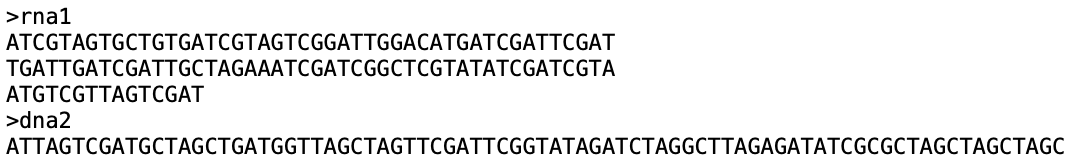
\includegraphics[width=0.8\textwidth]{figures/fasta-example.png}
%  \caption{Example of two FASTA sequence entries. One example with
%    sequence characters split across multiple lines, and one showing
%    all sequence characters on the same line.}
%  \label{fig:fasta-example}
%\end{figure}

%\subsection{FASTQ}
%Another popular sequencing format is the FASTQ format. This format is
%very similar to the FASTA format but with the addition of two more
%lines per sequence entry and a change to the character indicating the
%beginning of a new sequence entry. An example of a FASTQ entry is
%shown in figure~~\ref{fig:fastq-example}. In FASTQ formatted entries,
%the greater-than (\textgreater) character is swapped with the at (@)
%character. The evs for the sequence also follow a specific format,
%which provide information about the sequencing run and flowcell that
%the read was sequenced on. This information can then be traced back to
%the sequencing experiment in the case that there were errors or
%anomalies in the output from the experiment. Following the ID is the
%string of base calls. The evird line in a FASTQ entry is a plus (+)
%character, which indicates that the sequences character line has
%finished. Following the plus character is another sequence of
%characters, this time indicating the quality of basecall for the
%corresponding nucleotide base calls in the second line. The evality
%information included in FASTQ files are used to assess the quality of
%a sequencing run and extensively used in downstream processing steps,
%most notably in alignments.

%\begin{figure}
%  \centering
%  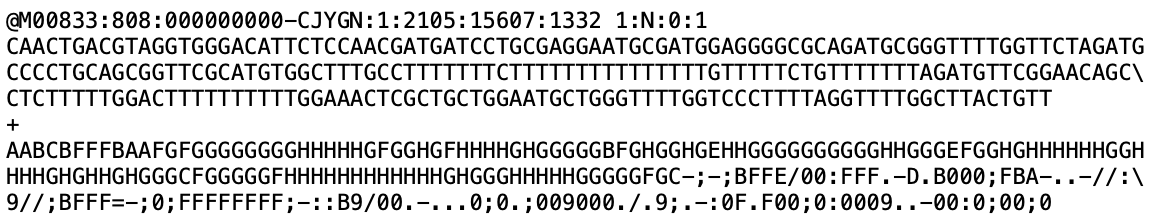
\includegraphics[width=0.8\textwidth]{figures/fastq-example.png}
%  \caption{Example of the four lines in a FASTQ entry.}
%  \label{fig:fastq-example}
%\end{figure}

%\subsection{General Feature Format - GFF}
%General feature format (GFF) is a popular format for storing
%information about features relative to a position on an genetic
%sequence, and comprises a large portion of annotation results from
%this work. These features can be whatever the user desires, as long as
%the feature entry follows the required GFF guidelines. Relative to a
%reference sequence, each GFF entry contains the following
%tab-delimited columns: sequence ID, source, feature type, start
%position, end position, score, strand, phase, and a semi-colon
%delimited list of attributes. GFF files are widely supported accross
%bioinformatics tools, making them highly versatile while also
%remaining relatively simple in nature but also allowing for storage of
%more complicated items via the attributes column. One significatn
%useage of GFF files is in visualization of features against the
%reference sequence from which they were derived. Most genome viewers
%(or browsers) support GFF files as input, allowing intuitive
%visualization of many features when overlayed on a reference
%sequence. An example of a GFF entry can be seen in
%figure~~\ref{fig:gff-example}.

%\begin{figure}
%  \centering
%  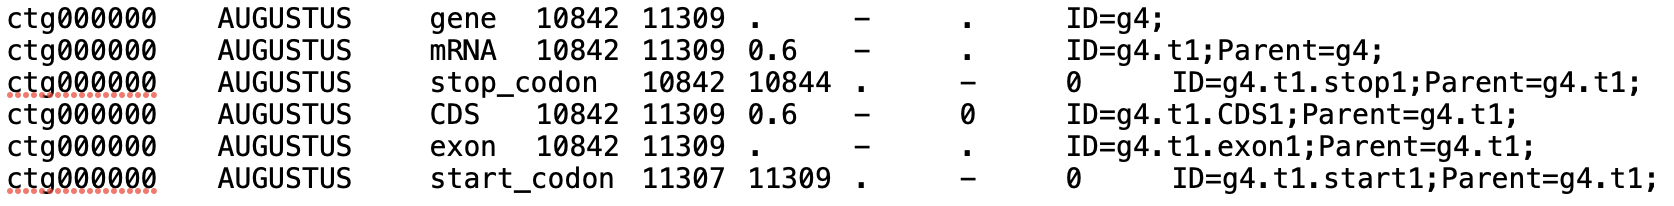
\includegraphics[width=0.8\textwidth]{figures/gff-example.png}
%  \caption{An example of GFF entries for a single gene.}
%  \label{fig:gff-example}
%\end{figure}

%\section{BLAST and tblastn}
%The evsic local	alignment search tool (BLAST)~\ref{Altschul1990}	has
%been a popular tool in the bioinformatics space, used to align
%biological sequences and measure their similarity. The eviginal	blast
%program was developed for alignment of nucleotide sequences, but other
%blast tools have been developed as well. One of these tools is tblastn
%which was developed to align reverse-translated protein sequences to
%another nucleotide sequence. To align the protein sequences, the query
%nucleotide sequences are translated in all six reading frames and then
%aligned to the proteins.  Tblastn is particularly useful for
%identifying functional or conserved proteins in	a nucleotide sequence.

%\section{BUSCO}
%The evnchmarking Universal Single-Copy Orthologs
%(BUSCO)~\ref{10.1093/bioinformatics/btv351} tool was developed to
%evaulate assemblies and subsequent annotations from the perspective of
%gene orthology. As genomes diverge evolutionarily, it is expected that
%some genes will be conserved as they are required for basic
%function. The evSCO (Benchmarking Universal Single-Copy Orthologs)
%tool and datasets were developed to assess completeness of an
%annotation in comparison to evolutionarily conserved genes.


\chapter{Results}
\section{Assemblies of DC1 and Tsth20}

Prior to assembly of DC1 and Tsth20 sequences, the tool FastQC was
used to evaluate the quality of the Illumina sequences provided for
this project. After trimming the Illumina sequences for low quality
reads, one FAIL flag was raised for both samples. This was the
per-sequence GC content flag, indicating that the GC content of
high-quality did not meet expectations. Plots of GC content for the
trimmed R1 sequences of both DC1 and Tsth20 are shown in
figure~\ref{fig:fastqc-lowgc}. In these plots, there is a considerable
increase in the number of sequences with GC content between 2 and 30\%,
which is important to note for later results and discussion.

\begin{figure}
  \centering
  \begin{subfigure}{0.8\textwidth}
    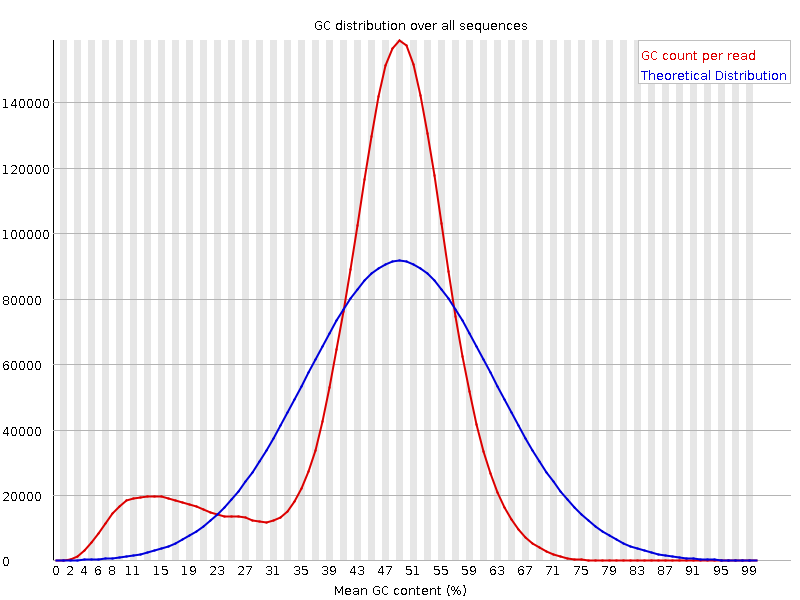
\includegraphics[width=\textwidth]{/Users/cbe453/Desktop/masters/masters/masters/working-thesis/figures/dc1-low-gc-fastqc.png}
    \caption{DC1}
    \label{fig:dc1fastqc}
  \end{subfigure}
  \\
  \begin{subfigure}{0.8\textwidth}
    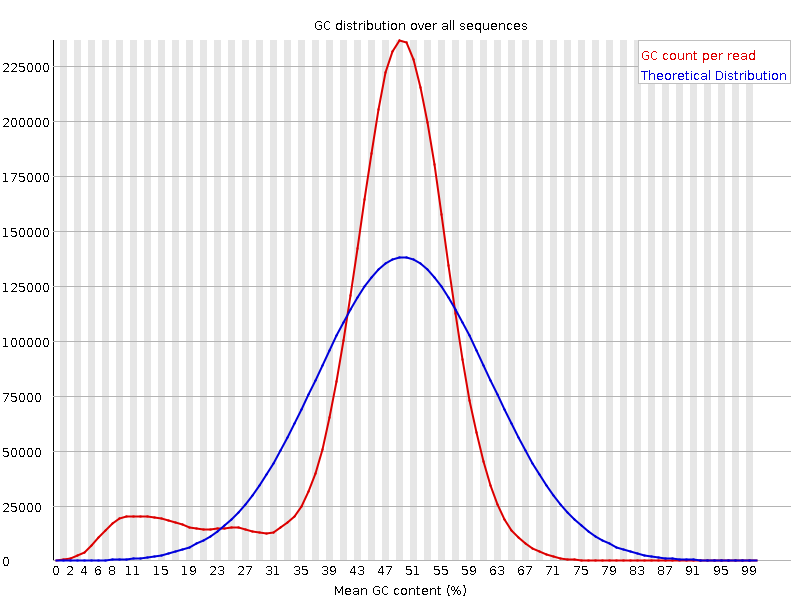
\includegraphics[width=\textwidth]{/Users/cbe453/Desktop/masters/masters/masters/working-thesis/figures/tsth20-low-gc-fastqc.png}
    \caption{Tsth20}
    \label{fig:tsth20fastqc}
  \end{subfigure}
  \caption{Plots showing the distribution of GC content in Illumina
    sequences.}
  \label{fig:fastqc-lowgc}
\end{figure}

A sliding window analysis was also performed on all final assemblies
in order to identify regions of anomalous GC content. The results of
this analysis are shown in figure~\ref{fig:assembly-gc}. Of the
included assemblies, anomalous GC content was identified in DC1,
Tsth20, \textit{T. reesei} and \textit{T. harzianum}, with
\textit{T. virens} showing no anomalous GC content. In addition to the
confirmation of anomalous GC content, it appears that the distribution
of GC content in \textit{T. reesei} differs from the other assemblies.

\begin{figure}
  \begin{center}
    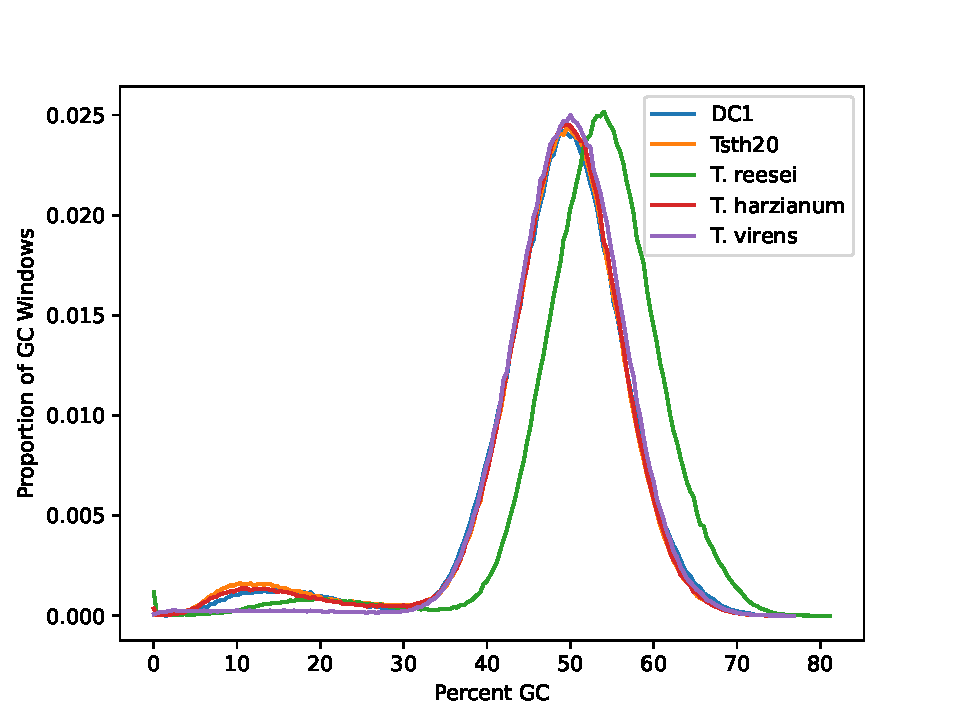
\includegraphics[width=0.8\textwidth]{figures/gc-plot.pdf}
  \end{center}
  \caption{Plots showing the frequency of GC values calculated from
    sliding windows for each assembly.}
  \label{fig:assembly-gc}
\end{figure}

For other general assembly metrics, the QUAST tool was used. Results
from QUAST are shown in figure~\ref{table:assemblies}, from which we can
make several observations. The most obvious observation to start with
is total contig counts for each assembly. For DC1 and Tsth20, the
total contig counts are an order of magnitude smaller when compared to
the other NCBI RefSeq assemblies, inidicating highly contiguous
assemblies from nextDenovo and nextPolish. This is likely due to the
use of long-read sequencing used in the assemblies of DC1 and
Tsth20. The total assembly lengths are similar, hovering around the
38-42Mb range, except in the case of \textit{T. reesei}, which is
known to have a significantly smaller genome length (ref) at roughly
33Mb. The largest contig size for each assembly vary greatly. DC1 and
Tsth20 have the largest contigs of all assemblies being considered,
which is again likely due to the inclusion of long-read sequencing
data in the assembly process. The N50 values for all assemblies are
above 1Mb, with DC1 and Tsth20 N50s being at minimum three times
larger than others assemblies.


\begin{table}
  \begin{center}
    \begin{tabular}{|c|c|c|c|c|c|c|}
      \hline
      Strain & Total Contigs & Total Length & Largest Contig & GC\% & N50 & L50 \\ \hline
      DC1 & 8 & 38.6 Mb & 11.49 Mb & 47.97 & 5.69 Mb & 3 \\ \hline
      Tsth20 & 7 & 41.58 Mb & 8.02 Mb & 47.33 & 6.52 Mb & 3 \\ \hline
      \textit{T. harzianum} & 532 & 40.98 Mb & 4.08 Mb & 47.61 & 2.41 Mb & 7 \\ \hline
      \textit{T. virens} & 93 & 39.02 Mb & 3.45 Mb & 49.25 & 1.83 Mb & 8 \\ \hline
      \textit{T. reesei} & 77 & 33.39 Mb & 3.75 Mb & 52.82 & 1.21 Mb & 9 \\ \hline
    \end{tabular}
  \end{center}
  \caption{General assembly metrics produced by QUAST (a
    genome quality assement tool).}
  \label{table:assemblies}
\end{table}



\section{Initial Gene Finding Results} 
\label{section:gene-finding}

Prior to discussing gene finding results, we will first define the
terms gene and coding sequence in the context of this work. We refer
to a gene as a set of start and stop coordinates in a genomic
sequence. This definition of a gene simplifies processing, although
the definition could be expanded in the future to include introns,
exons and potential up and downstream sequences as well. Gene finders
may also predict isoforms, or alternative splice variants of a gene
based on evidence provided in training, resulting in multiple
potential coding sequences for a gene. In this work, we refer to
coding sequences as the set of all coding sequences predicted by a
gene finder.

Counts of genes and coding sequences predicted by Braker2, GeneMark
and RefSeq are shown in Figure~\ref{fig:gene-counts}, Figure~\ref{fig:cds-counts} and Table~\ref{table:gene-counts}. Immediately we
see that Braker2 predicts far fewer genes in all assemblies, except in
the case of \textit{Trichoderma reesei.} This is possibly due to the
effects of training the Braker2 gene model using data from
\textit{Trichoderma reesei}, which has a significantly smaller genome
in comparison to other \textit{Trichoderma} assemblies, although
genome size is not always indicative of gene content. Regardless, we
observe a difference in the number of genes predicted by Braker2 in
comparison to GeneMark and RefSeq. The number of genes predicted by
GeneMark and RefSeq are similar, except in the case of
\textit{T. harzianum}, in which RefSeq predicts roughly 17\% more
genes than GeneMark. Braker2 consistently predicts more coding
sequences than GeneMark and RefSeq. RefSeq also appears to predict
multiple coding sequences for each gene but in fewer numbers than
Braker2. Coding sequence prediction counts in \textit{T. harzianum}
from RefSeq are also interesting, with RefSeq predicting fewer coding
sequences than genes. Why this occurs is unknown but may warrant
further investigation.

\begin{figure}
  \centering
  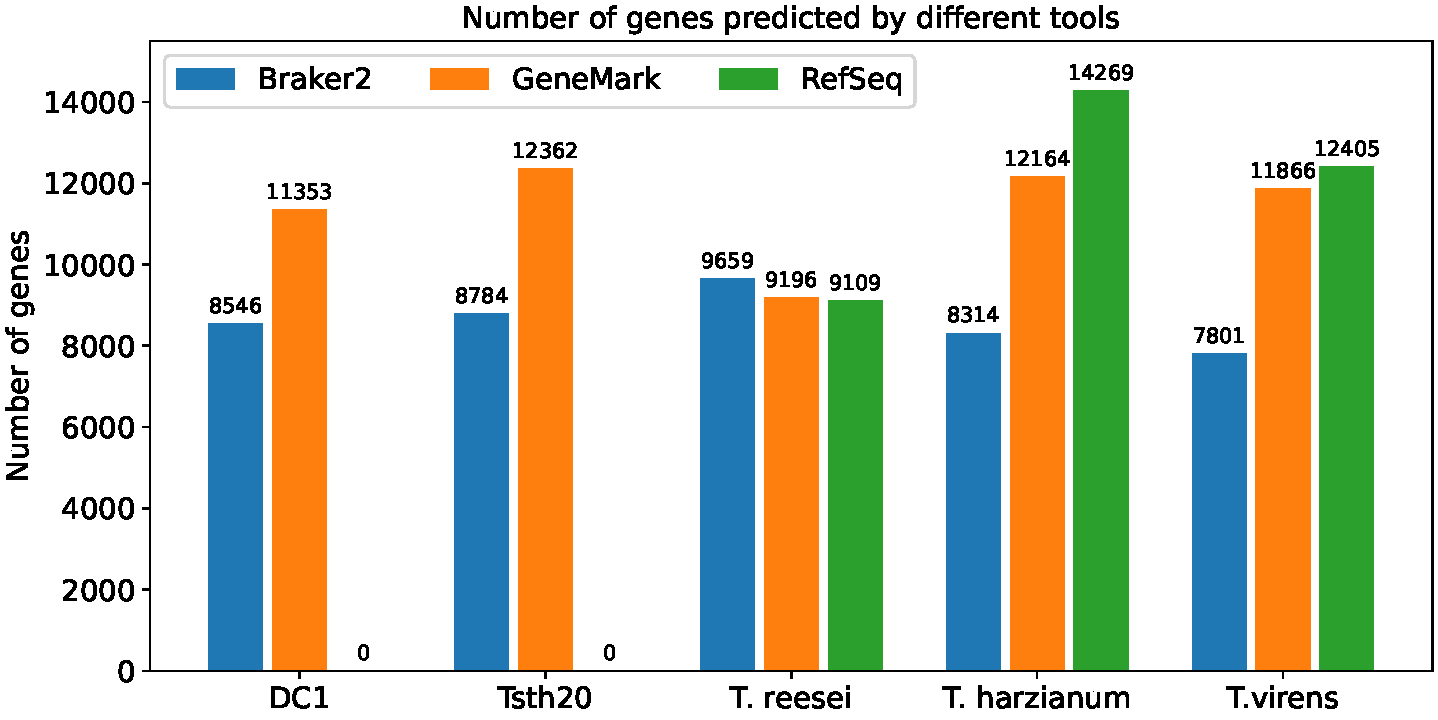
\includegraphics[width=0.9\textwidth]{figures/gene-counts-barplot.pdf}
  \caption[Number of genes predicted]{Number of genes predicted by each gene finder for each \textit{Trichoderma} genome assembly.}
  \label{fig:gene-counts}
\end{figure}

\begin{figure}
  \centering
  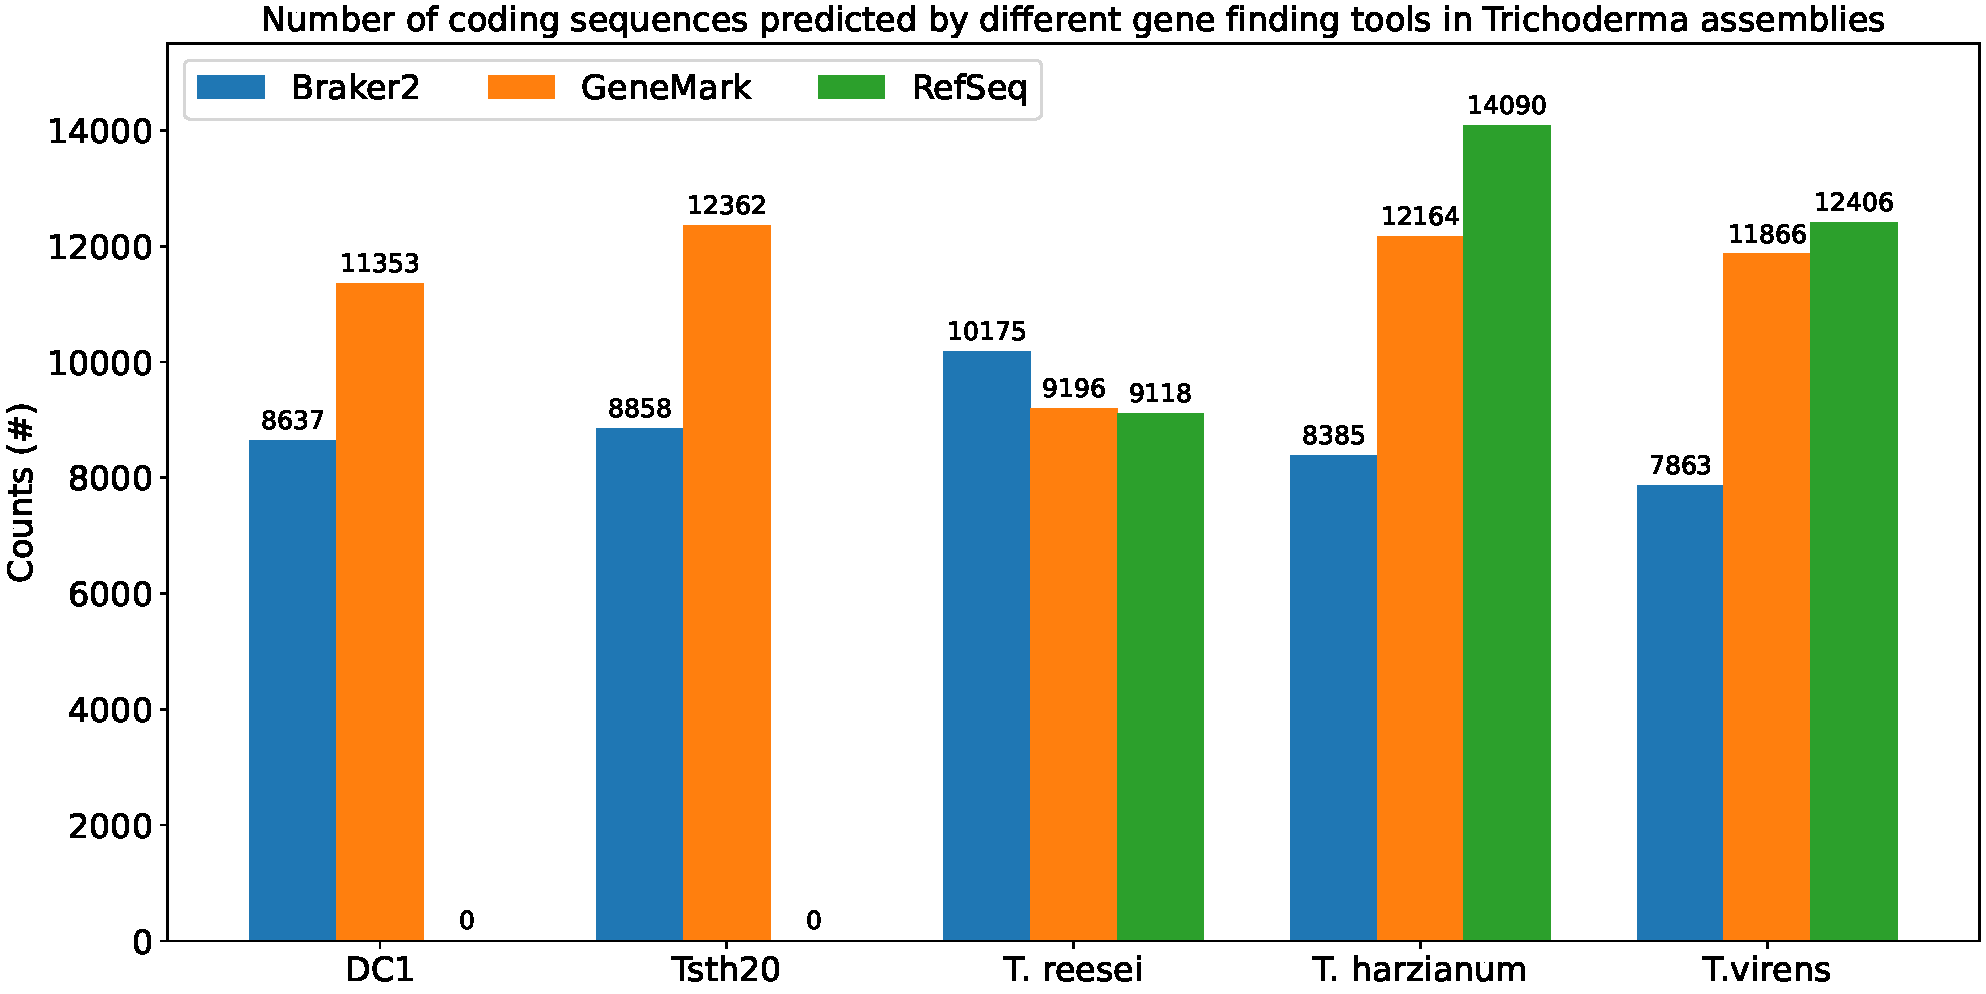
\includegraphics[width=0.9\textwidth]{figures/cds-counts-barplot.pdf}
  \caption[Number of coding sequences predicted]{Number of coding sequences predicted by each gene finder for each \textit{Trichoderma} genome assembly.}
  \label{fig:cds-counts}
\end{figure}

\begin{table}
  \centering
  \begin{tabular}{|c|c|c|c|c|c|c|}
    \hline
    Assembly & Braker2 & & GeneMark & & RefSeq & \\ \hline
     & Genes & CDS & Genes & CDS & Genes & CDS \\ \hline
    DC1 & 8546 & 8637 & 11353 & 11353 & N/A & N/A \\ \hline
    Tsth20 & 8784 & 8858 & 12362 & 12362 & N/A & N/A \\ \hline
    \textit{T. reesei} & 9659 & 10175 & 9196 & 9196 & 9109 & 9118 \\ \hline
    \textit{T. harzianum} & 8314 & 8385 & 12164 & 12164 & 14269 & 14090 \\ \hline
    \textit{T. virens} & 7801 & 7863 & 11866 & 11866 & 12405 & 12406 \\ \hline
  \end{tabular}
  \caption[Gene prediction counts]{Number of genes and coding sequences
    (isoforms) predicted by each gene finder for each
    \textit{Trichoderma} genome.}
  \label{table:gene-counts}
\end{table}



\section{Region Identification}
\label{section:regions}

Visual breakdowns of the types of regions identified and their counts
for each \textit{Trichoderma} assembly are shown in figure
\ref{fig:regions-sankey}. We will discuss the types of regions,
beginning with fully supported regions. These regions, labelled `Full
Support', are sections of genomic sequence where each gene finder
agrees that a gene is present in some form. These fully supported
regions are then broken down into two categories, based on whether or
not the models from each gene finder agree on the start and/or stop
positions of the gene model. Regions that have support from more than
one gene finder, but not all, are labelled regions with `Partial
Support'. These regions are also broken down in to two subtypes based
on whether or not the gene predictions agree on the start and/or stop
positions of the gene. Regions with support from only one gene finder
are labelled as singletons.

\begin{figure}
  \centering
  \begin{subfigure}{0.9\textwidth}
    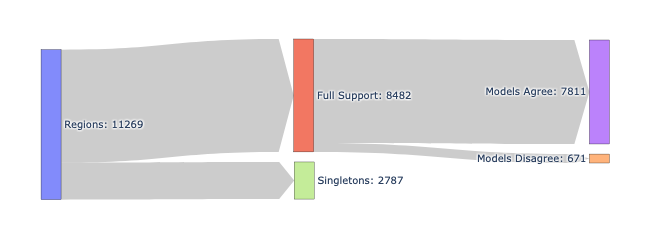
\includegraphics[width=\textwidth]{figures/dc1-region-breakdown.png}
    \label{fig:dc1-regions}
    \caption{DC1}
  \end{subfigure}
  \begin{subfigure}{0.9\textwidth}
    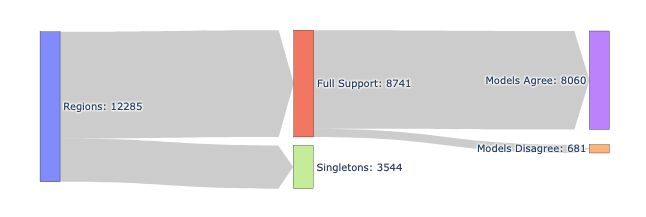
\includegraphics[width=\textwidth]{figures/tsth20-region-breakdown.png}
    \label{fig:tsth20-regions}
    \caption{Tsth20}
  \end{subfigure}
  \begin{subfigure}{0.9\textwidth}
    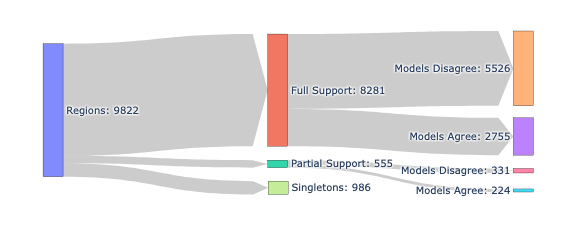
\includegraphics[width=\textwidth]{figures/t-reesei-region-breakdown.png}
    \label{fig:t-reesei-regions}
    \caption{\textit{T. reesei}}
  \end{subfigure}
\end{figure}
\begin{figure}
  \ContinuedFloat
  \centering
  \begin{subfigure}{0.9\textwidth}
    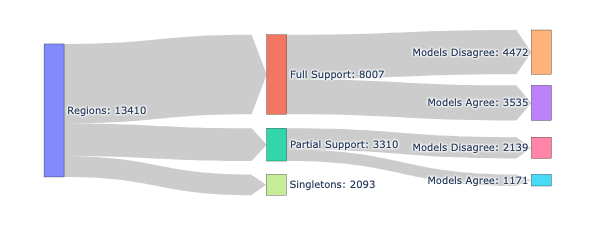
\includegraphics[width=\textwidth]{figures/t-harzianum-region-breakdown.png}
    \label{fig:t-harzianum-regions}
    \caption{\textit{T. harzianum}}
  \end{subfigure}
  \begin{subfigure}{0.9\textwidth}
    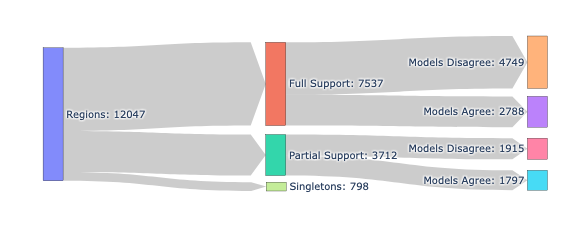
\includegraphics[width=\textwidth]{figures/t-virens-region-breakdown.png}
    \label{fig:t-virens-regions}
    \caption{\textit{T. virens}}
  \end{subfigure}
  \caption[Breakdown of identified regions]{Figures showing breakdowns
    of genomic regions identified by the region finding
    process. Regions, in blue, are categorized based on support from
    gene finders. Regions with supporting predictions from all gene
    finders included in this analysis are labelled with `Full Support'
    and colored red. Fully supported regions are then broken down into
    regions where gene models agree on the start and stop positions of
    the genes (purple), and those that do not (orange). Regions
    labelled with `Partial Support' (turquoise) are regions with
    supporting gene predictions from more than one gene finder, but
    not all. Partially supported regions are also broken down into
    regions in which gene finders agree on the start and stop
    positions of the gene (cyan), and those that do not agree
    (pink). Regions with gene predictions from only one gene finder
    are labelled as singletons (green).}
  \label{fig:regions-sankey}
\end{figure}

Looking at DC1 and Tsth20 in figure \ref{fig:regions-sankey}, it
appears that Braker2 and GeneMark predict genes in the same regions in
the majority of cases. For regions with full support, the models also
tend to agree on the start and stop positions of the gene in that
region. This is not generally the case as we will see later. There are
no regions with partial support for DC1 and Tsth20, as there are only
two gene finders considered, leaving only complete agreement or
disagreement. \textit{Trichoderma reesei} contains the fewest number
of regions, which seems to scale appropriately with the total number
of predicted genes and assembly length. The vast majority of the
regions are fully or partially supported by Braker2, GeneMark and
RefSeq, with only 10 percent of the regions being single
predictions. The most interesting observation here is the number of
fully supported regions that disagree on start and stop positions of
the gene(s) in each region. There is clearly a difference in the gene
models being produced by these gene finders. If there is also more
disagreement on the start and stop positions of a gene, then there is
likely disagreement on the number and location of exons and introns
within the gene model as well. In the case of partially supported
regions, there is more disagreement than agreement, but that may come
as less of a surprise as there is already disgreement on presence by
definition. Gene finding behaviour in regions from
\textit{T.harzianum} and \textit{T. virens} differ from the other
assemblies in the split between fully and partially supported
regions. There seems to be fewer regions with full support from all
gene finders and the reason why is unclear. The gene models in each
region, whether fully or partially supported, still tend to disagree
on start and stop positions of the genes more often than agree.

It is also worthwhile investigating some potentially interesting cases
of strange gene calls in regions. One such case is when a region
contains more than three individual predicted genes. The null
hypothesis, so to speak, is that if all gene finders agree exactly on
the presence and position of a gene in a region, then one should
expect exactly three predictions in that region. We observe that this
is not always true. Cases of more than three gene predictions in a
region were present in regions from all processed assemblies. Figure
\ref{fig:uncertain-regions} shows an example of one of these regions,
in which the single gene predicted by RefSeq spans multiple gene
predictions from both Braker2 and GeneMark. In the case of DC1 and
Tsth20, there were very few regions that matched this scenario, with
19 and 6 regions matching, respectively. Conversly, \textit{T. reesei,
  T.harzianum and T.virens} contain many such regions, with assemblies
reporting 546, 899 and 521 regions with greater than three gene
predictions, respectively. While having predictions from each gene
finding tool present in a region is a strong indicator for the
presence of a gene, having more than one gene prediction per gene
finder raises questions about which model (or models) is correct and
why disagreement exists.

\begin{figure}
  \centering
  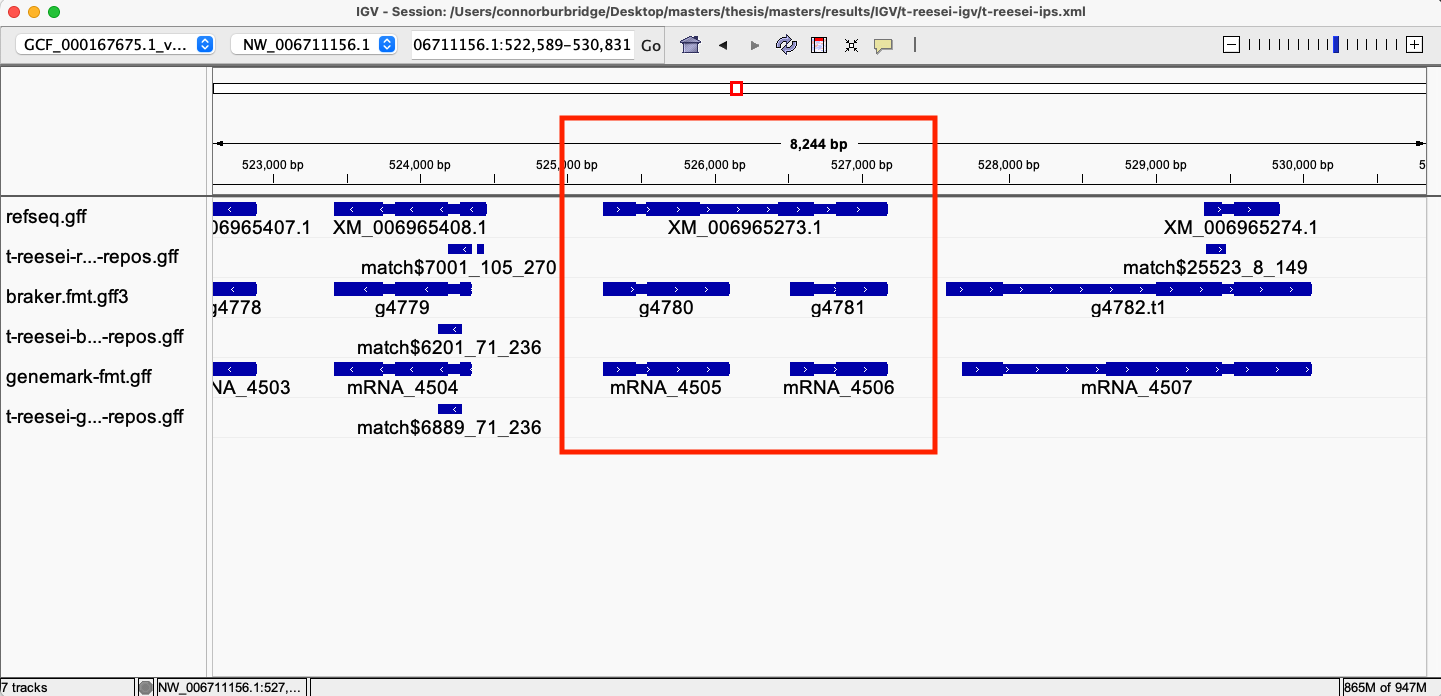
\includegraphics[width=0.9\textwidth]{figures/igv/igv-uncertain-regions.png}
  \caption[Example of a region with many gene calls]{An IGV screenshot
    from \textit{T. reesei} showing a region containing five
    gene predictions.}
  \label{fig:uncertain-regions}
\end{figure}

Another interesting set of criteria to investigate is whether or not
gene finders always predict genes on the same strand within a
region. We observe that regions containing predictions on different
strands do exist, and are observed in predictions from all assemblies
included in this analysis. Figure \ref{fig:opposing-strands} shows an
example of a region containing gene predictions on opposing
strands. As in the case of regions with more than three gene
predictions, DC1 and Tsth20 report fewer mixed strand regions with DC1
reporting 29 regions and Tsth20 reporting 46. \textit{T. reesei,
  T. harzianum and T. virens} report more regions in which this
property is true, with region counts being 203, 533 and 293
respectively. Under the assumption that gene finders should predict
the same genes on the same strands, it is unexpected to find so many
of these cases, and will require further investigation.

\begin{figure}
  \centering
  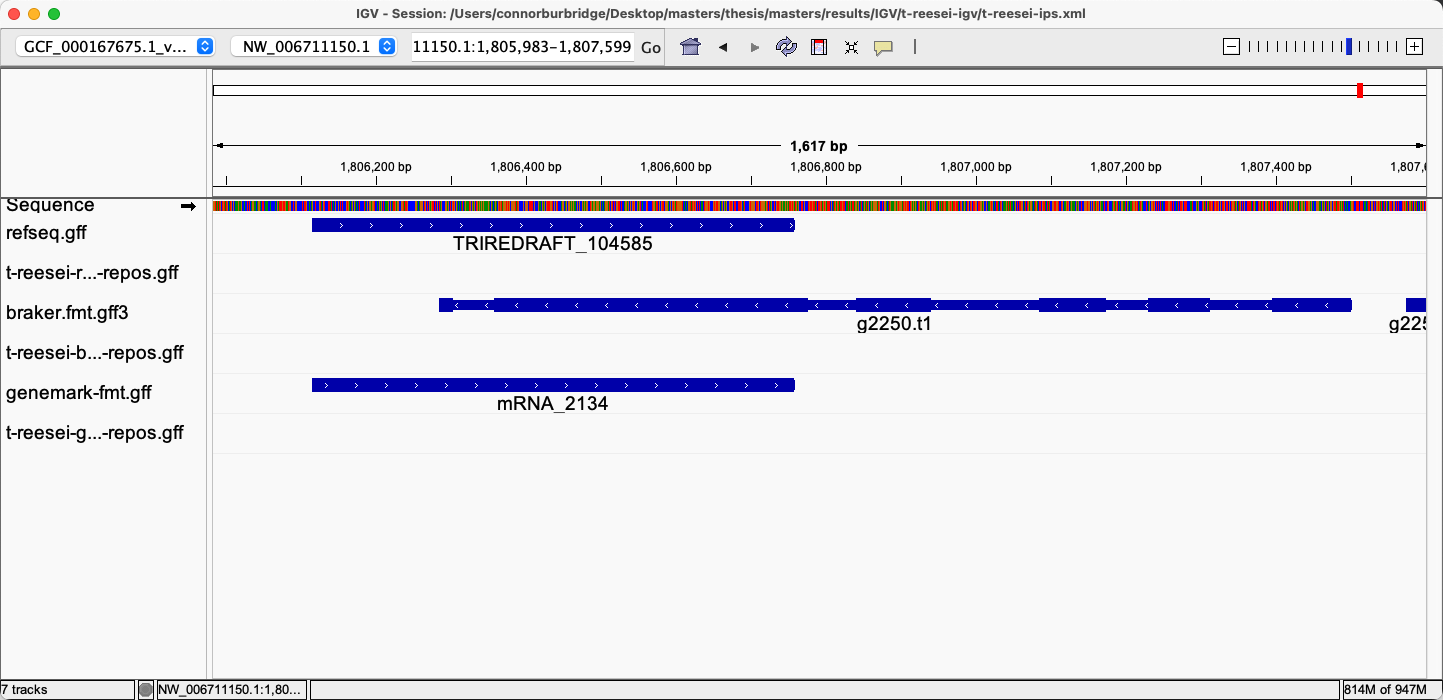
\includegraphics[width=0.9\textwidth]{figures/igv/igv-opposing-strands.png}
  \caption[Predictions on opposing strands]{An IGV screenshot of
    \textit{T. reesei} showing a region which contains gene
    predictions on opposite strands.}
  \label{fig:opposing-strands}
\end{figure}

In summary, gene finders agree partially or completely on the presence
of a gene in the vast majority of cases. While gene finders generally
agree on the presence of a gene, they tend to disagree on the
underlying gene model more often than they agree, except in in the
case of DC1 and Tsth20. This is likely due to only including two gene
finders in their analysis rather than three, resulting in fewer
opportunities for disagreement. This observation is true when applied
to the start and stop positions of the gene, but further investigation
and comparison of intronic and exonic sequences between genes may
provide more insight. Finally, regions identified in this analysis do
not always fit the ideal scenario of one gene prediction from each
tool per region. Regions in which there are more than three gene
predictions were observed in all assemblies included in this work. In
addition, gene finders do not always predict genes on the same strand
as other gene finders.

\section{BUSCO Results}
\label{section:busco}

Results of BUSCO analysis using the sordariomycetes\_Odb12 dataset provided by BUSCO are presented in Figure~\ref{fig:busco-complete}, Figure~\ref{fig:busco-missing}, and Table~\ref{table:busco}. The results 
indicate that all gene sets considered in this analysis have a BUSCO
completeness of 94.9\% or higher, with a maximum completeness of
99.9\% in the case of Braker2 and DC1. In general, Braker2 and RefSeq have the
most BUSCO complete sets of gene predictions of the three tools
considered. Interestingly, Braker2 produces far more duplicated BUSCO
matches than both GeneMark and RefSeq. Examining the BUSCO output
logs, this appears to be due to Braker2 predicting more than one
coding sequence for some genes predictions, resulting in multiple
similar proteins. Interestingly, the coding sequences in the RefSeq annotations seem to miss far more genes than the other two gene finders while also having a higher number of fragmented BUSCO genes. This may be due to human curation of the RefSeq datasets, or the Gnomon gene prediction pipeline used by NCBI to produce these annotations. Further investigation is required to determine the exact cause of this discrepancy. Finally, it appears that \textit{T. reesei} tends to have slightly lower BUSCO completeness than the other \textit{Trichoderma} species considered in this analysis, regardless of gene finder used. Why this is the case is unknown, but may be due to the evolutionary distance between \textit{T. reesei}, the Gnomon annotation process, or potentially the fragmented nature of the \textit{T. reesei} assembly used in this analysis. 

In general, all gene finders perform
well in regards to BUSCO performance. While these results do not
capture the entire set of genes possibly present in these
\textit{Trichoderma} assemblies, they do confirm that the gene finders
are at minimum predicting many evolutionarily conserved fungal genes.

\begin{figure}
  \centering
  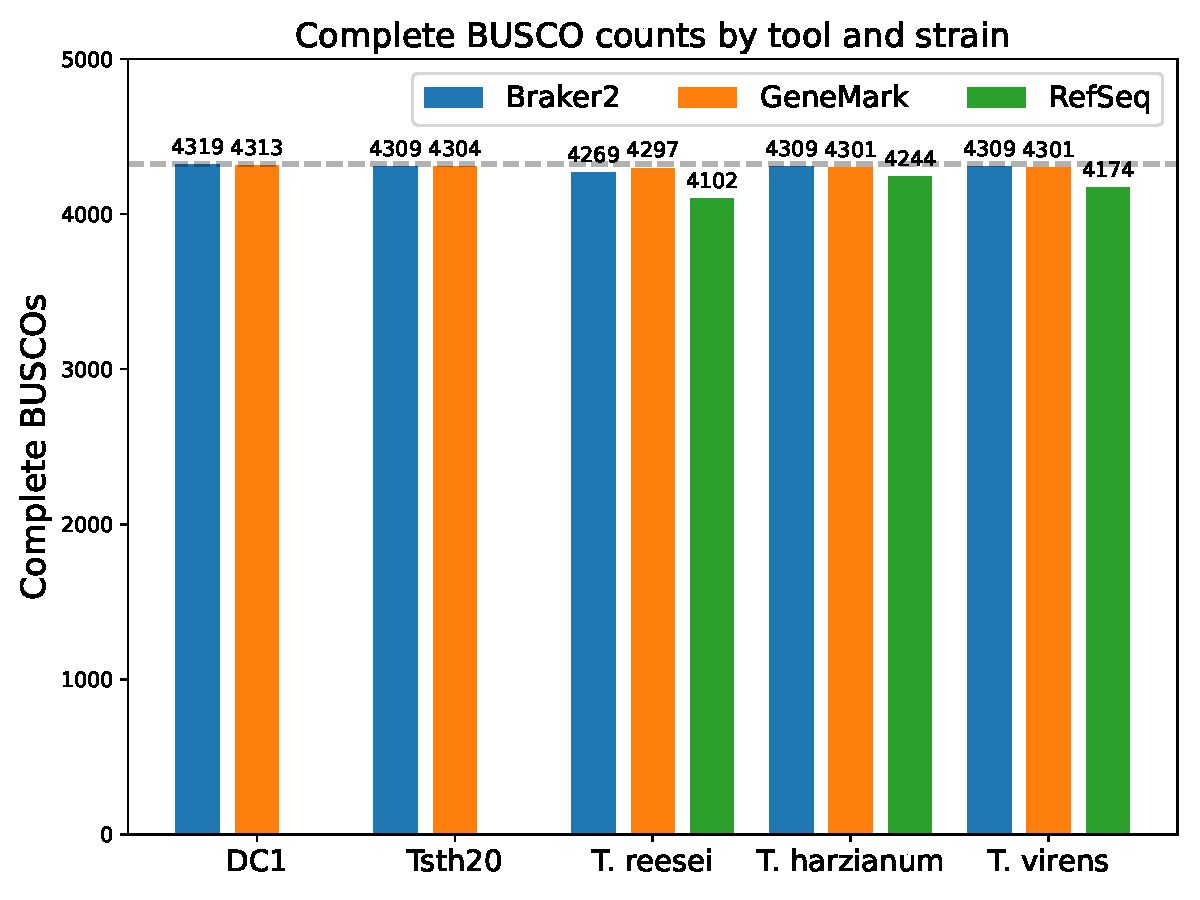
\includegraphics[width=0.90\textwidth]{figures/busco-complete-counts.pdf}
  \caption[Complete BUSCO counts]{Barplot showing the number of complete BUSCOs for each gene finder across all \textit{Trichoderma} genome assemblies. For DC1 and Tsth20, RefSeq annotations are not available, so their values are set to 0. The dashed line indicates the total number of BUSCO markers in the selected dataset (4323).}
  \label{fig:busco-complete}
\end{figure}

\begin{figure}
  \centering
  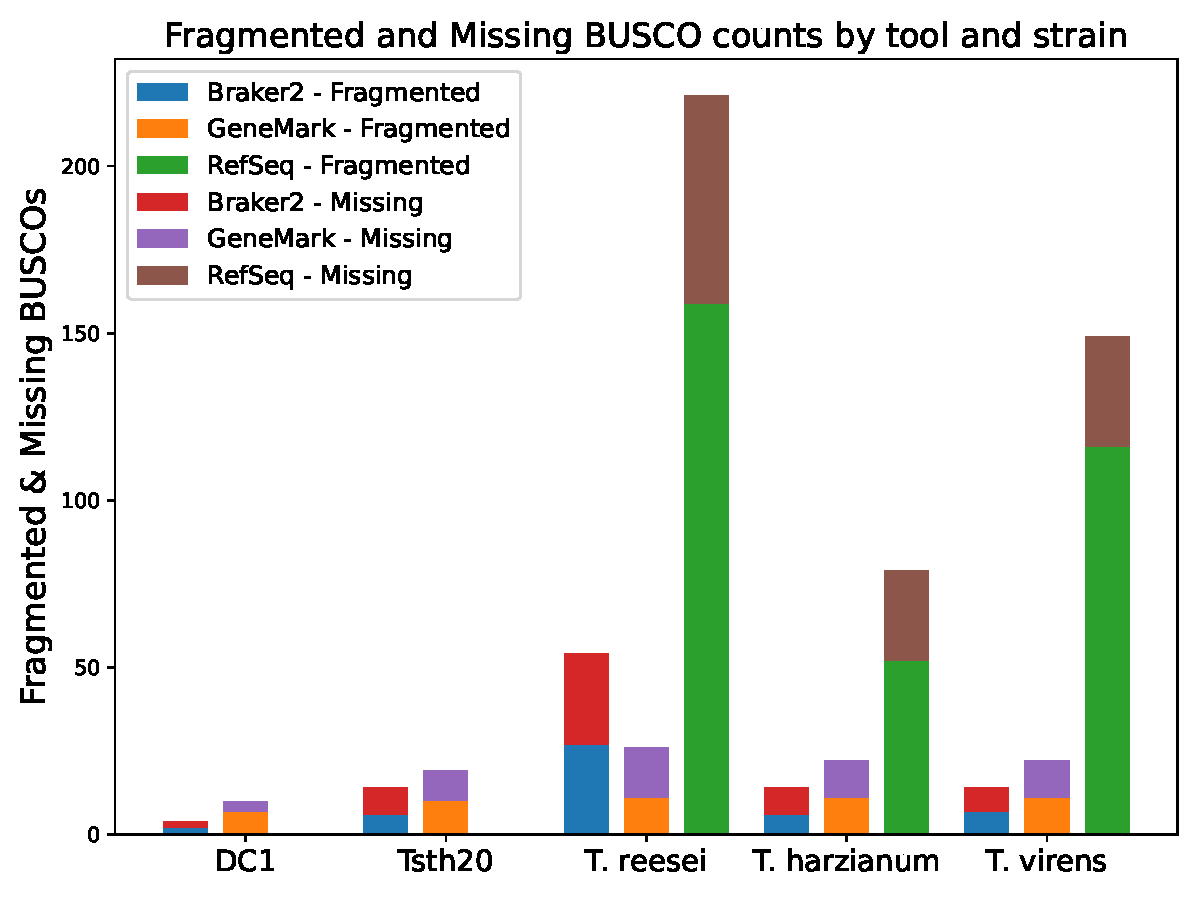
\includegraphics[width=0.90\textwidth]{figures/busco-missing-counts.pdf}
  \caption[Missing BUSCO counts]{Barplot showing the number of missing BUSCOs for each gene finder across all \textit{Trichoderma} genome assemblies. For DC1 and Tsth20, RefSeq annotations are not available, so their values are set to 0. The dashed line indicates the total number of BUSCO markers in the selected dataset (4323).}
  \label{fig:busco-missing}
\end{figure}

\begin{table}
  \begin{center}
    \begin{subtable}{\textwidth}
      \centering
      \begin{tabular}{|c|c|c|c|c|c|c|}
        \hline
        Strain & Complete & Single & Duplicated & Fragmented & Missing \\ \hline
        DC1 & 4319 & 3505 & 814 & 2 & 2 \\ \hline
        Tsth20 & 4309 & 3575 & 734 & 6 & 8 \\ \hline
        \textit{T. reesei} & 4269 & 3616 & 653 & 27 & 27 \\ \hline
        \textit{T. harzianum} & 4309 & 3562 & 747 & 6 & 8 \\ \hline
        \textit{T. virens} & 4309 & 3504 & 805 & 7 & 7 \\ \hline
      \end{tabular}
      \caption{Braker2}
      \vspace{0.5cm}
    \end{subtable}
    \begin{subtable}{\textwidth}
      \centering
      \begin{tabular}{|c|c|c|c|c|c|c|}
        \hline
        Strain & Complete & Single & Duplicated & Fragmented & Missing \\ \hline
        DC1 & 4313 & 4311 & 2 & 7 & 3 \\ \hline
        Tsth20 & 4304 & 4291 & 13 & 10 & 9 \\ \hline
        \textit{T. reesei} & 4297 & 4297 & 0 & 11 & 15 \\ \hline
        \textit{T. harzianum} & 4301 & 4291 & 10 & 11 & 11 \\ \hline
        \textit{T. virens} & 4301 & 4291 & 10 & 11 & 11 \\ \hline
      \end{tabular}
      \caption{GeneMark}
      \vspace{0.5cm}
    \end{subtable}
    \begin{subtable}{\textwidth}
      \centering
      \begin{tabular}{|c|c|c|c|c|c|c|}
        \hline
        Strain & Complete & Single & Duplicated & Fragmented & Missing \\ \hline
        \textit{T. reesei} & 4102 & 4101 & 1 & 159 & 62 \\ \hline
        \textit{T. harzianum} & 4244 & 4234 & 10 & 52 & 27 \\ \hline
        \textit{T. virens} & 4174 & 4164 & 10 & 116 & 33 \\ \hline  
      \end{tabular}
      \caption{RefSeq}
    \end{subtable}
  \end{center}
  \caption{Results from BUSCO using the fungal analysis option
    organized by gene finding tool. The selected BUSCO dataset
    contains 4323 markers. For more information on the categories
    assigned by BUSCO, please refer to the documentation.}
  \label{table:busco}
\end{table}

While BUSCO matches are a good metric for general performance of gene
finders, it is also important to investigate BUSCO proteins without
matching gene predictions. Table \ref{table:busco}, shows breakdowns
of genes missed by each gene finder across the \textit{Trichoderma}
assemblies. 


%\begin{center}
% \begin{table}
% \makebox[\textwidth]{
% \begin{tabular}{|c|c|c|c|c|c|c|c|}
%   \hline
%   Tool & BUSCO ID & Annotation & DC1 & Tsth20 & \textit{T. reesei} & \textit{T. harzianum} & \textit{T. virens} \\ \hline
%   Braker2 & 195619at4751 & \makecell{Pyridoxal phosphate-dependent \\ transferase} & \  & \checkmark & \checkmark & \checkmark & \checkmark \\ \hline
%   Braker2 & 285254at4751 & Aminoacyl-tRNA synthetase & \checkmark & \checkmark & \checkmark &  & \checkmark \\ \hline
%   Braker2 & 348020at4751 & Formyl transferase &  &  & \checkmark &  & \checkmark \\ \hline
%   Braker2 & 497024at4751 & Zinc finger C2H2-type &  & \checkmark & \checkmark & \checkmark & \checkmark \\ \hline
%   GeneMark & 195619at4751 & \makecell{Pyridoxal phosphate-dependent \\ transferase} &  & \checkmark & \checkmark & \checkmark & \checkmark \\ \hline
%   GeneMark & 285254at4751 & Aminoacyl-tRNA synthetase & \checkmark & \checkmark & \checkmark &  & \checkmark \\ \hline
%   GeneMark & 348020at4751 & Formyl transferase &  &  &  &  & \checkmark \\ \hline 
%   GeneMark & 438731at4751 & LSM domain & \checkmark & \checkmark &  & \checkmark & \checkmark  \\ \hline
%   GeneMark & 470813at4751 & Ubiquitin-conjugating enzyme &  &  &  &  &  \\ \hline
%   GeneMark & 497024at4751 & Zinc finger C2H2-type &  & \checkmark & \checkmark & \checkmark & \checkmark \\ \hline
%   RefSeq & 494at4751 & Midasin & N/A & N/A &  &  & \checkmark\\ \hline
%   RefSeq & 315802at4751 & tRNA dimethylallyltransferase & N/A & N/A & \checkmark & \checkmark &  \\ \hline
%   RefSeq & 352224at4751 & YEATS & N/A & N/A &  & \checkmark &  \\ \hline
% \end{tabular}
% }
% \caption[GeneMark missed BUSCO proteins]{The presence (\checkmark)
%   or absence of all BUSCO IDs missed by Braker2, GeneMark and RefSeq
%   in each \textit{Trichoderma} assembly.}
% \label{table:genemark-busco}
%\end{table}
%\end{center}

%\begin{table}
%  \centering
%  \begin{tabular}{|c|c|c|c|c|c|c|}
%    \hline
%    BUSCO ID & Annotation & DC1 & Tsth20 & \textit{T. reesei} & \textit{T. harzianum} & \textit{T. reesei} \\ \hline
%    494at4751 & Midasin & N/A & N/A & X & X & \checkmark\\ \hline
%    315802at4751 & tRNA dimethylallyltransferase & N/A & N/A & \checkmark & \checkmark & X \\ \hline
%    352224at4751 & YEATS & N/A & N/A & X & \checkmark & X \\ \hline
%  \end{tabular}
%  \caption[RefSeq missed BUSCO proteins]{The presence (\checkmark) or
%    absence (X) of all BUSCO IDs missed by RefSeq in each
%    \textit{Trichoderma} assembly.}
%  \label{table:refseq-busco}
%\end{table}

Braker2, GeneMark and RefSeq all demonstrate excellent coverage of the
BUSCO fungal protein set, indicating that these gene finders are
capable of predicting genes that are expected to be present in these
assemblies. From this we can say that the foundations of the
underlying gene models used by each gene finder are solid. Braker2
produces more duplicate matches than GeneMark and RefSeq, but this is
likely due to multiple isoforms of possible genes being present in the
input data. Despite excellent coverage of the BUSCO fungal proteins,
all three gene finders miss some BUSCO proteins in their
predictions. 
Finally, we reiterate the possibility that human curation of RefSeq datasets is responsible for these differences, but this requires further investigation.


\chapter{Discussion}
\section{Assemblies of DC1 and Tsth20}
Overall, the assemblies of DC1 and Tsth20 resulted in what can be
described as sequences suitable for further downstream
processing. Assembled lengths for both samples are similar to closely
related \textit{Trichoderma} accessions, indicating that the
assemblies are of appropriate length, but this could be confirmed with
further wetlab experiments in the future. The assembly of DC1 resulted
in eight contigs, with two sequences, ctg000040 being significantly
shorter at 65Kb than it's counterparts, which deviates from the
expected 7 chromosome-scale contigs expected from a
\textit{Trichoderma} assembly\cite{Kubicek2019}. Why this sequence is
significantly shorter than other contigs is unclear, but could arise
for several reasons. The most obvious reason would be mis-assembly,
which could arise from complications caused by both the anomolous GC
content reginos as well as highly repetitive regions. Even with the
inclusion of Nanopore sequencing data, it is possible that there was
insufficient support for connection between these contigs and
others. This highlights the complexity of assembling sequences with
anomolous content and supports the idea that multiple rounds and forms
of sequencing data may be required to produce scaffold and reference
level assemblies of non-model organisms. Another possible explanation
for an unaccounted for contig could be the assembly of a mitochondrial
genome, although this appears somewhat unlikely due to the length of
the ctg000040, it is not entirely out of the question. Previous work
focusing on mitochondrial genomes in \textit{Trichoderma} shows the
lengths of mitochondrial assemblies from six \textit{Trichoderma}
samples to be between 27Kb and 42Kb.

The assembly of Tsth20 resulted in seven contigs, matching that of the
expected seven chromosomes detected in most \textit{Trichoderma}
strains. The total assembled length of Tsth20 is again similar but
slightly larger than existing \textit{Trichoderma} assemblies.

\section{Initial Gene Counts}
Initial gene counts from Braker2 and Genemark show a similar trend in
all assemblies included in this analysis. Braker tends to predict
fewer genes in comparison to GeneMark and RefSeq results except in the
case of \textit{T. reesei}. The cause of this difference is likely
two-fold in nature. Most importantly, Braker2 was trained on an RNAseq
dataset derived from \textit{T. reesei}. This additional information
in the gene finding model is likely why Braker2 finds more genes and
transcripts than GeneMark. The effects of this training set may also
be why Braker2 tends to predict fewer genes and transcripts in other
assemblies when compared to results from GeneMark and RefSeq. The
nature of gene models in \textit{T. reesei} likely differs than those
of other genomes, resulting in 'poorer' relative performance than in
\textit{T. reesei}. This highlights the fact that users should choose
training sets carefully when planning to use a hybrid gene finding
approach. Choosing a dataset that is inappropriate will end with
results that are skewed or biased towards the training set of
interest, although they will likely be of higher confidence. This is
an important trade-off to consider when preparing for a hybrid gene
finding approach.

Another potential explanation of Braker2's low gene count trend could
again be due to the reference training set used in training. However
in this case, not necessarily due to the RNAseq data itself, but the
nature and size of the genome from whih the RNAseq data was gathered
from. The \textit{T. reesei} genome is significantly smaller than
other assemblies considered as shown in figure (blah), resulting in
less physical space for coding sequences to be found. This would
explain why GeneMark predicts a similar number of genes as Braker2 in
\textit{T. reesei} but not in any of the other assemblies. In theory,
it would make sense that after training, Braker2 would predict a
fraction of all possible genes in a larger assembly, since it was
trained with RNAseq data from a genome that is a fraction of the
size. Again, this shows that the choice of training data is paramount
when planning a hybrid assembly approach to gene finding.



\section{BUSCO Analysis}

The results from BUSCO analysis of the gene sets produced by each
prediction method prove promising. With all gene sets being 99.2\%
complete or higher based on the fungal dataset provided to BUSCO. This
higher number indicates that these gene finding tools capture nearly
completely the set of evolutionarily conserved single-copy orthologs
pre-defined by BUSCO curators. In the case of the fungal dataset,
there are 758 genes considered during analysis.

The most glaring observation from this analysis is the duplication
level found in the gene sets produced by Braker2 in comparison to the
GeneMark and RefSeq datasets. The Braker gene sets show a single-copy
match for roughly 80-85\% of the total gene call set with duplicates
making up the other 15-20\% of the set. The likliest reason for this
difference is the presence of isoforms in gene sets produced by
Braker. As shown in figure \ref{fig:genecounts}, Braker2 does produce
isoforms in it's output, which would be identified as duplicates in
the BUSCO process. However, the number of isoforms predicted per gene
does not make up 20\% of the total set of gene calls. It is possible
that the BUSCO dataset contains a large fraction of the Braker2 gene
calls with isoforms, but that is unlikely and warrants further
investigation into the genes matching the BUSCO dataset.  Another
possible explanation is that Braker2 is predicting genes that are
actually isoforms as separate genes. BUSCO also makes note of isoforms
of a gene being the cause of high number of duplicates, and recommends
users remove isoforms prior to running BUSCO, although that step was
not performed for this work.





\chapter{Results}
\section{Assemblies of DC1 and Tsth20}

Prior to assembly of DC1 and Tsth20 sequences, the tool FastQC was
used to evaluate the quality of the Illumina sequences provided for
this project. After trimming the Illumina sequences for low quality
reads, one FAIL flag was raised for both samples. This was the
per-sequence GC content flag, indicating that the GC content of
high-quality did not meet expectations. Plots of GC content for the
trimmed R1 sequences of both DC1 and Tsth20 are shown in
figure~\ref{fig:fastqc-lowgc}. In these plots, there is a considerable
increase in the number of sequences with GC content between 2 and 30\%,
which is important to note for later results and discussion.

\begin{figure}
  \centering
  \begin{subfigure}{0.8\textwidth}
    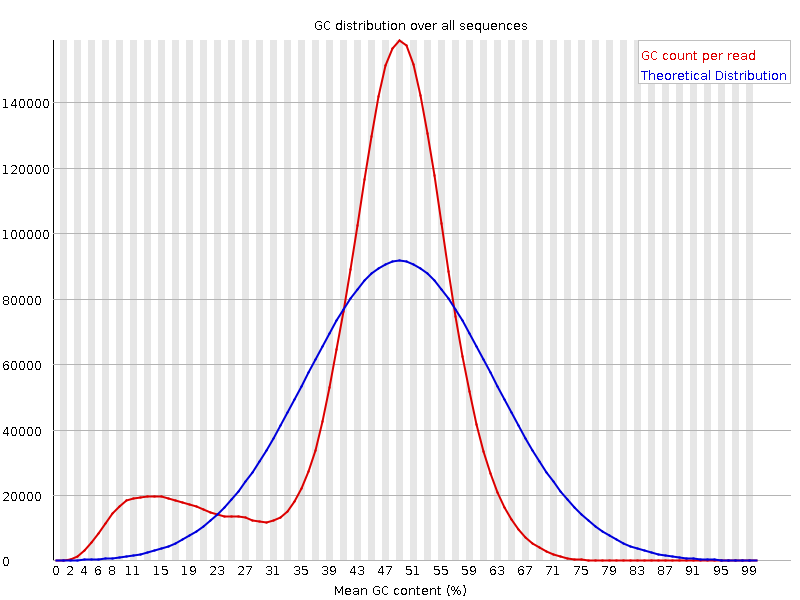
\includegraphics[width=\textwidth]{/Users/cbe453/Desktop/masters/masters/masters/working-thesis/figures/dc1-low-gc-fastqc.png}
    \caption{DC1}
    \label{fig:dc1fastqc}
  \end{subfigure}
  \\
  \begin{subfigure}{0.8\textwidth}
    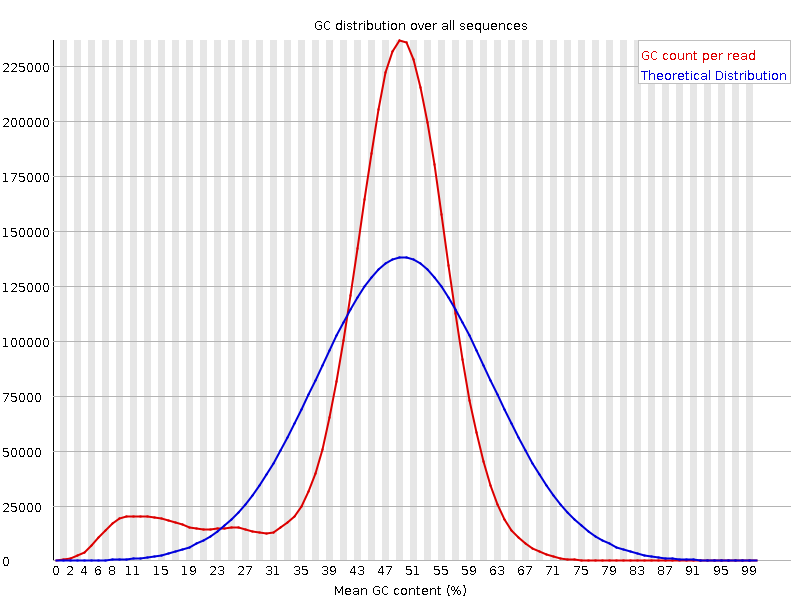
\includegraphics[width=\textwidth]{/Users/cbe453/Desktop/masters/masters/masters/working-thesis/figures/tsth20-low-gc-fastqc.png}
    \caption{Tsth20}
    \label{fig:tsth20fastqc}
  \end{subfigure}
  \caption{Plots showing the distribution of GC content in Illumina
    sequences.}
  \label{fig:fastqc-lowgc}
\end{figure}

A sliding window analysis was also performed on all final assemblies
in order to identify regions of anomalous GC content. The results of
this analysis are shown in figure~\ref{fig:assembly-gc}. Of the
included assemblies, anomalous GC content was identified in DC1,
Tsth20, \textit{T. reesei} and \textit{T. harzianum}, with
\textit{T. virens} showing no anomalous GC content. In addition to the
confirmation of anomalous GC content, it appears that the distribution
of GC content in \textit{T. reesei} differs from the other assemblies.

\begin{figure}
  \begin{center}
    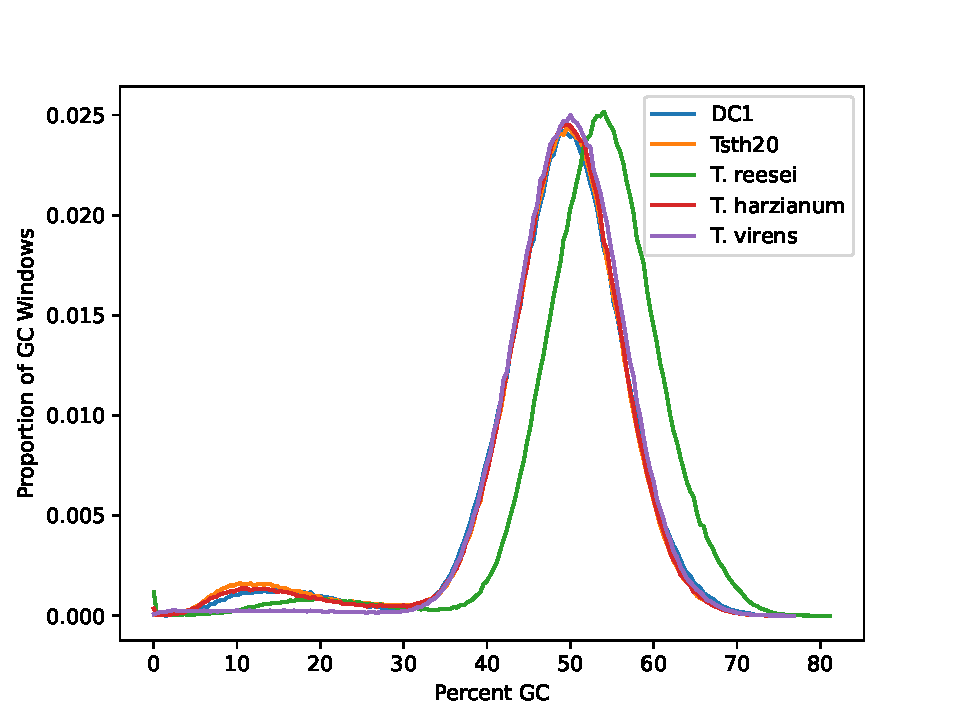
\includegraphics[width=0.8\textwidth]{figures/gc-plot.pdf}
  \end{center}
  \caption{Plots showing the frequency of GC values calculated from
    sliding windows for each assembly.}
  \label{fig:assembly-gc}
\end{figure}

For other general assembly metrics, the QUAST tool was used. Results
from QUAST are shown in figure~\ref{table:assemblies}, from which we can
make several observations. The most obvious observation to start with
is total contig counts for each assembly. For DC1 and Tsth20, the
total contig counts are an order of magnitude smaller when compared to
the other NCBI RefSeq assemblies, inidicating highly contiguous
assemblies from nextDenovo and nextPolish. This is likely due to the
use of long-read sequencing used in the assemblies of DC1 and
Tsth20. The total assembly lengths are similar, hovering around the
38-42Mb range, except in the case of \textit{T. reesei}, which is
known to have a significantly smaller genome length (ref) at roughly
33Mb. The largest contig size for each assembly vary greatly. DC1 and
Tsth20 have the largest contigs of all assemblies being considered,
which is again likely due to the inclusion of long-read sequencing
data in the assembly process. The N50 values for all assemblies are
above 1Mb, with DC1 and Tsth20 N50s being at minimum three times
larger than others assemblies.


\begin{table}
  \begin{center}
    \begin{tabular}{|c|c|c|c|c|c|c|}
      \hline
      Strain & Total Contigs & Total Length & Largest Contig & GC\% & N50 & L50 \\ \hline
      DC1 & 8 & 38.6 Mb & 11.49 Mb & 47.97 & 5.69 Mb & 3 \\ \hline
      Tsth20 & 7 & 41.58 Mb & 8.02 Mb & 47.33 & 6.52 Mb & 3 \\ \hline
      \textit{T. harzianum} & 532 & 40.98 Mb & 4.08 Mb & 47.61 & 2.41 Mb & 7 \\ \hline
      \textit{T. virens} & 93 & 39.02 Mb & 3.45 Mb & 49.25 & 1.83 Mb & 8 \\ \hline
      \textit{T. reesei} & 77 & 33.39 Mb & 3.75 Mb & 52.82 & 1.21 Mb & 9 \\ \hline
    \end{tabular}
  \end{center}
  \caption{General assembly metrics produced by QUAST (a
    genome quality assement tool).}
  \label{table:assemblies}
\end{table}



\section{Initial Gene Finding Results} 
\label{section:gene-finding}

Prior to discussing gene finding results, we will first define the
terms gene and coding sequence in the context of this work. We refer
to a gene as a set of start and stop coordinates in a genomic
sequence. This definition of a gene simplifies processing, although
the definition could be expanded in the future to include introns,
exons and potential up and downstream sequences as well. Gene finders
may also predict isoforms, or alternative splice variants of a gene
based on evidence provided in training, resulting in multiple
potential coding sequences for a gene. In this work, we refer to
coding sequences as the set of all coding sequences predicted by a
gene finder.

Counts of genes and coding sequences predicted by Braker2, GeneMark
and RefSeq are shown in Figure~\ref{fig:gene-counts}, Figure~\ref{fig:cds-counts} and Table~\ref{table:gene-counts}. Immediately we
see that Braker2 predicts far fewer genes in all assemblies, except in
the case of \textit{Trichoderma reesei.} This is possibly due to the
effects of training the Braker2 gene model using data from
\textit{Trichoderma reesei}, which has a significantly smaller genome
in comparison to other \textit{Trichoderma} assemblies, although
genome size is not always indicative of gene content. Regardless, we
observe a difference in the number of genes predicted by Braker2 in
comparison to GeneMark and RefSeq. The number of genes predicted by
GeneMark and RefSeq are similar, except in the case of
\textit{T. harzianum}, in which RefSeq predicts roughly 17\% more
genes than GeneMark. Braker2 consistently predicts more coding
sequences than GeneMark and RefSeq. RefSeq also appears to predict
multiple coding sequences for each gene but in fewer numbers than
Braker2. Coding sequence prediction counts in \textit{T. harzianum}
from RefSeq are also interesting, with RefSeq predicting fewer coding
sequences than genes. Why this occurs is unknown but may warrant
further investigation.

\begin{figure}
  \centering
  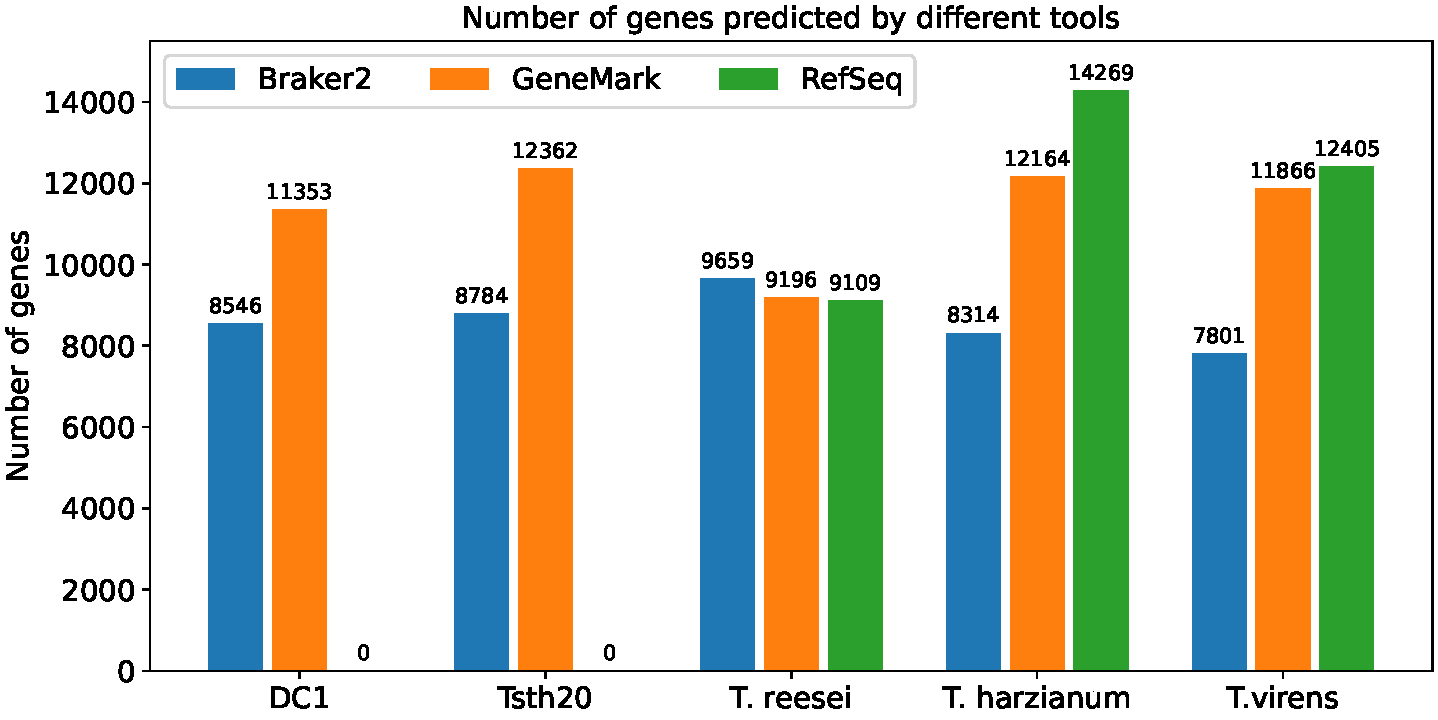
\includegraphics[width=0.9\textwidth]{figures/gene-counts-barplot.pdf}
  \caption[Number of genes predicted]{Number of genes predicted by each gene finder for each \textit{Trichoderma} genome assembly.}
  \label{fig:gene-counts}
\end{figure}

\begin{figure}
  \centering
  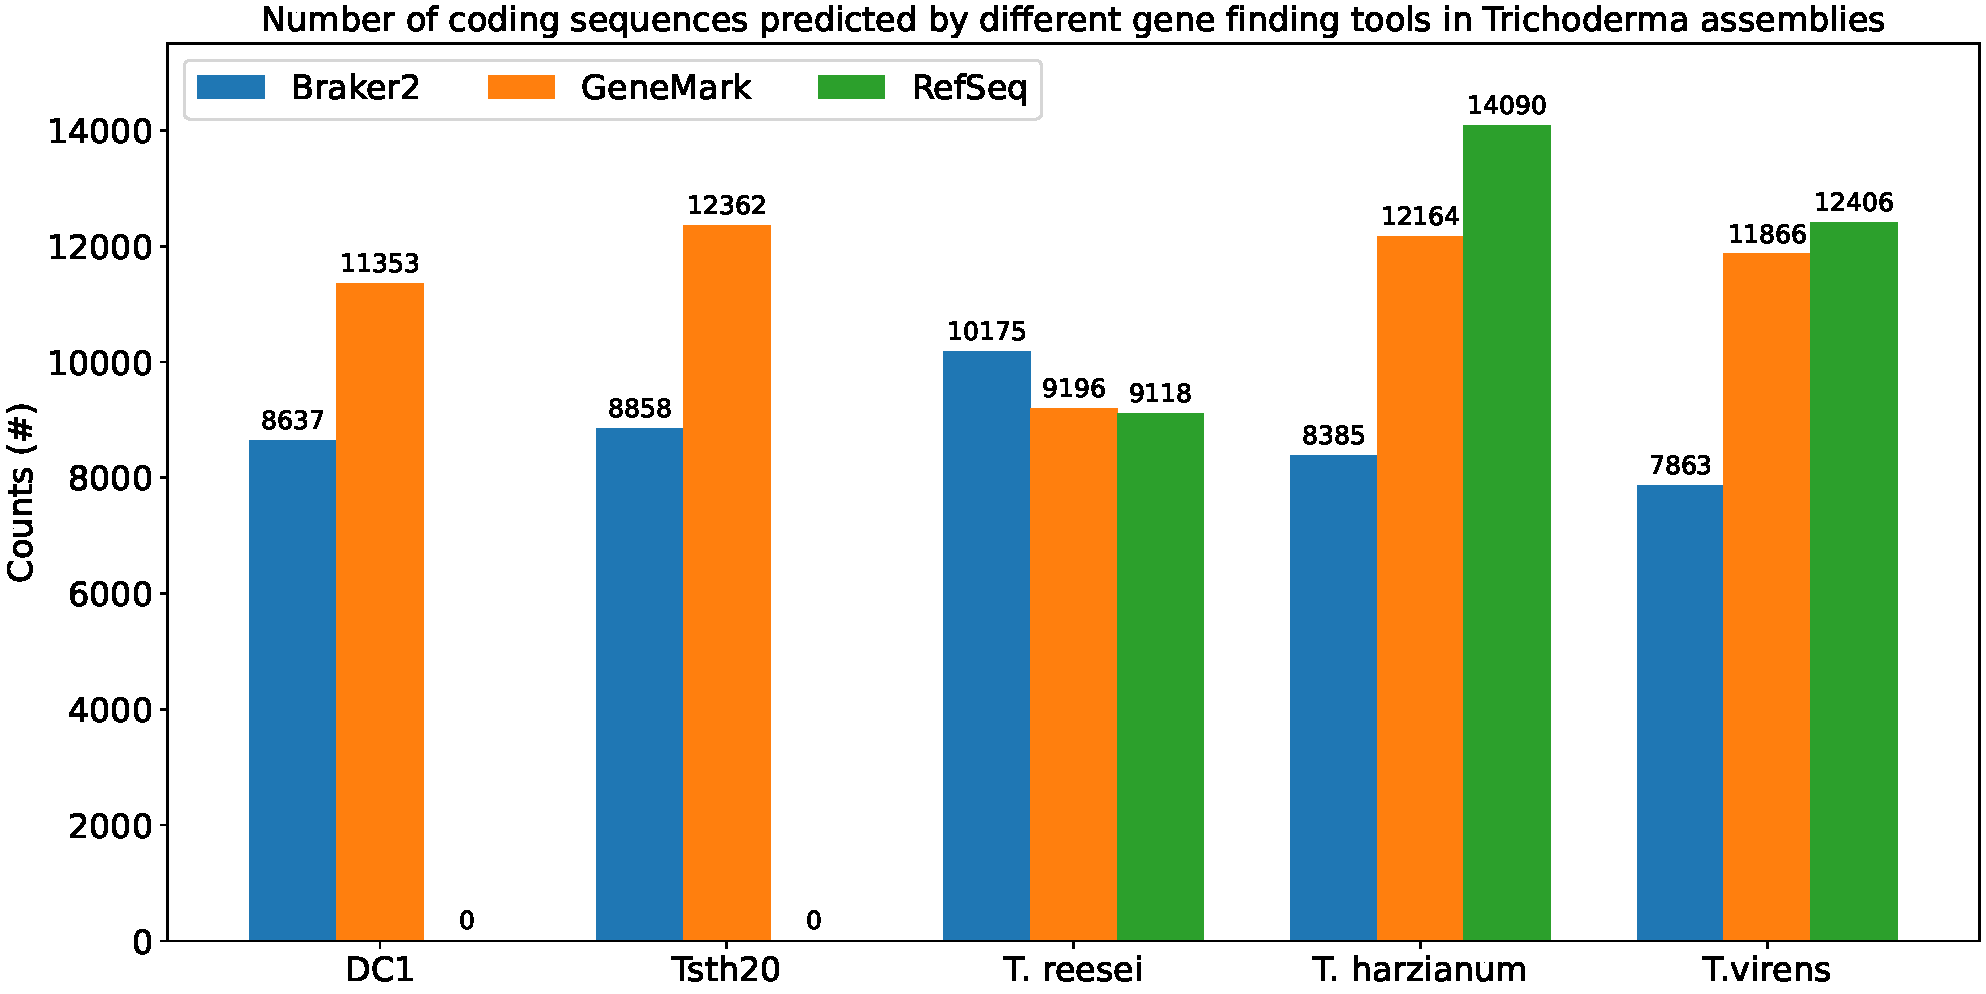
\includegraphics[width=0.9\textwidth]{figures/cds-counts-barplot.pdf}
  \caption[Number of coding sequences predicted]{Number of coding sequences predicted by each gene finder for each \textit{Trichoderma} genome assembly.}
  \label{fig:cds-counts}
\end{figure}

\begin{table}
  \centering
  \begin{tabular}{|c|c|c|c|c|c|c|}
    \hline
    Assembly & Braker2 & & GeneMark & & RefSeq & \\ \hline
     & Genes & CDS & Genes & CDS & Genes & CDS \\ \hline
    DC1 & 8546 & 8637 & 11353 & 11353 & N/A & N/A \\ \hline
    Tsth20 & 8784 & 8858 & 12362 & 12362 & N/A & N/A \\ \hline
    \textit{T. reesei} & 9659 & 10175 & 9196 & 9196 & 9109 & 9118 \\ \hline
    \textit{T. harzianum} & 8314 & 8385 & 12164 & 12164 & 14269 & 14090 \\ \hline
    \textit{T. virens} & 7801 & 7863 & 11866 & 11866 & 12405 & 12406 \\ \hline
  \end{tabular}
  \caption[Gene prediction counts]{Number of genes and coding sequences
    (isoforms) predicted by each gene finder for each
    \textit{Trichoderma} genome.}
  \label{table:gene-counts}
\end{table}



\section{BLAST Results}
Results from the T-BLAST-N runs are presented in table
\ref{table:tblastn}. Initial BLAST results appear promising for both
the \textit{T. atroviride} and \textit{Fusarium} datasets. All
assemblies considered contain at minimum 89\% of the reference protein
sequences in the case of \textit{T. atroviride} and a minimum of 75\%
in the case of \textit{Fusarium}. In the case of
\textit{S. cerevisiae}, a minimum of 57\% of reference proteins
matched. The decreasing percentage of hits reported conincides with
increasing distances in the evolutionary tree. These results provide
rough validation that the assemblies contain potential for protein
coding sequences.


\begin{table}
  \centering
  \begin{tabular}{|c|c|c|c|c|c|c|}
    \hline
    Reference & Ref. Proteins & DC1 & Tsth20 & \textit{T. reesei} & \textit{T. harzianum} & \textit{T. virens}  \\ \hline
    \textit{T. atroviride} & 11807 & 11552 & 11080 & 10601 & 11081 & 11078 \\ \hline 
    \textit{Fusarium} & 13312 & 10327 & 10429 & 10064 & 10434 & 10490 \\ \hline
    \textit{S. cerevisiae} & 6014 & 3537 & 3517 & 3445 & 3509 & 3500 \\ \hline
  \end{tabular}
  \caption{tBLASTn hits from reference protein sequences to selected
    assemblies of intereset. Hits are reported if the alignment length
    is greater than 30\% of the reference protein length and if 30\%
    of the aligned length have identical matches.}
  \label{table:tblastn}
\end{table}

\section{BUSCO Results}
\label{section:busco}

Results of BUSCO analysis using the sordariomycetes\_Odb12 dataset provided by BUSCO are presented in Figure~\ref{fig:busco-complete}, Figure~\ref{fig:busco-missing}, and Table~\ref{table:busco}. The results 
indicate that all gene sets considered in this analysis have a BUSCO
completeness of 94.9\% or higher, with a maximum completeness of
99.9\% in the case of Braker2 and DC1. In general, Braker2 and RefSeq have the
most BUSCO complete sets of gene predictions of the three tools
considered. Interestingly, Braker2 produces far more duplicated BUSCO
matches than both GeneMark and RefSeq. Examining the BUSCO output
logs, this appears to be due to Braker2 predicting more than one
coding sequence for some genes predictions, resulting in multiple
similar proteins. Interestingly, the coding sequences in the RefSeq annotations seem to miss far more genes than the other two gene finders while also having a higher number of fragmented BUSCO genes. This may be due to human curation of the RefSeq datasets, or the Gnomon gene prediction pipeline used by NCBI to produce these annotations. Further investigation is required to determine the exact cause of this discrepancy. Finally, it appears that \textit{T. reesei} tends to have slightly lower BUSCO completeness than the other \textit{Trichoderma} species considered in this analysis, regardless of gene finder used. Why this is the case is unknown, but may be due to the evolutionary distance between \textit{T. reesei}, the Gnomon annotation process, or potentially the fragmented nature of the \textit{T. reesei} assembly used in this analysis. 

In general, all gene finders perform
well in regards to BUSCO performance. While these results do not
capture the entire set of genes possibly present in these
\textit{Trichoderma} assemblies, they do confirm that the gene finders
are at minimum predicting many evolutionarily conserved fungal genes.

\begin{figure}
  \centering
  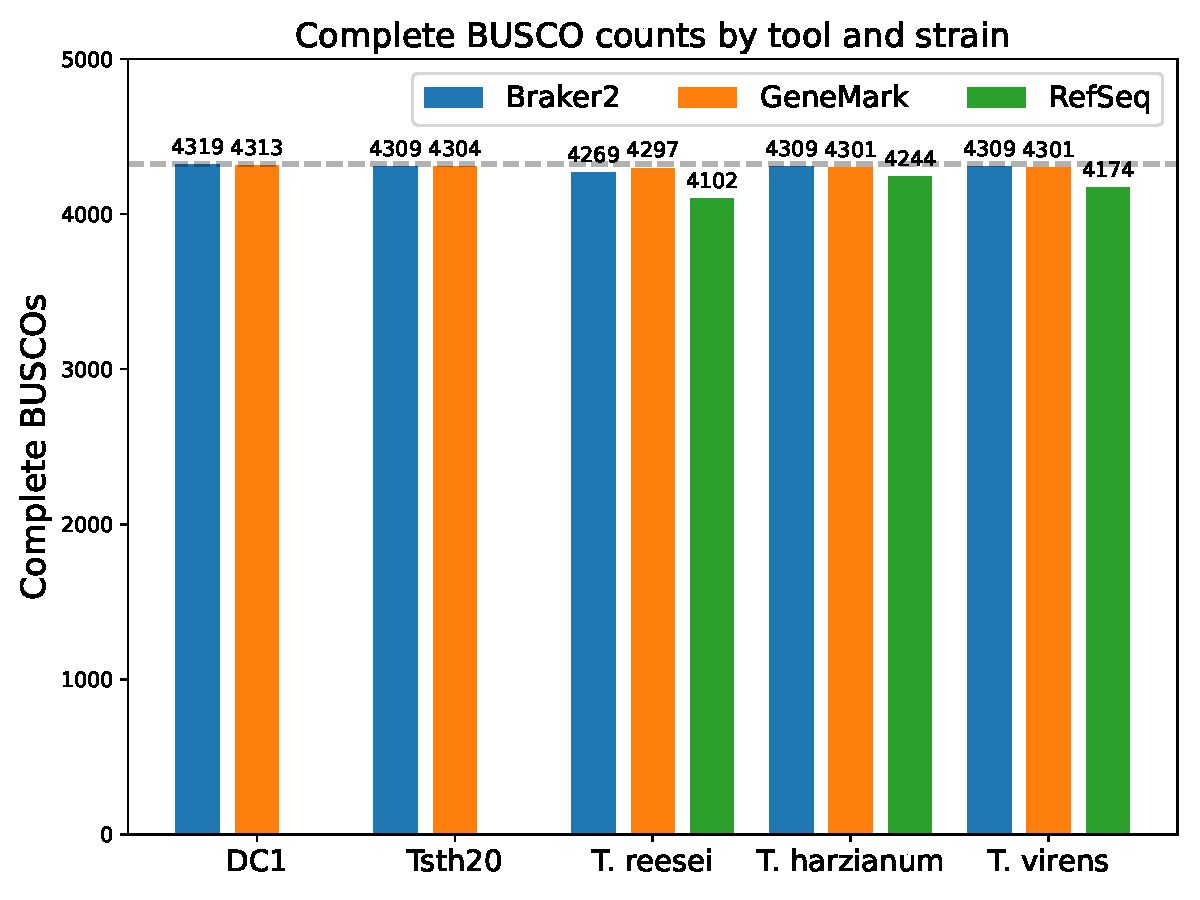
\includegraphics[width=0.90\textwidth]{figures/busco-complete-counts.pdf}
  \caption[Complete BUSCO counts]{Barplot showing the number of complete BUSCOs for each gene finder across all \textit{Trichoderma} genome assemblies. For DC1 and Tsth20, RefSeq annotations are not available, so their values are set to 0. The dashed line indicates the total number of BUSCO markers in the selected dataset (4323).}
  \label{fig:busco-complete}
\end{figure}

\begin{figure}
  \centering
  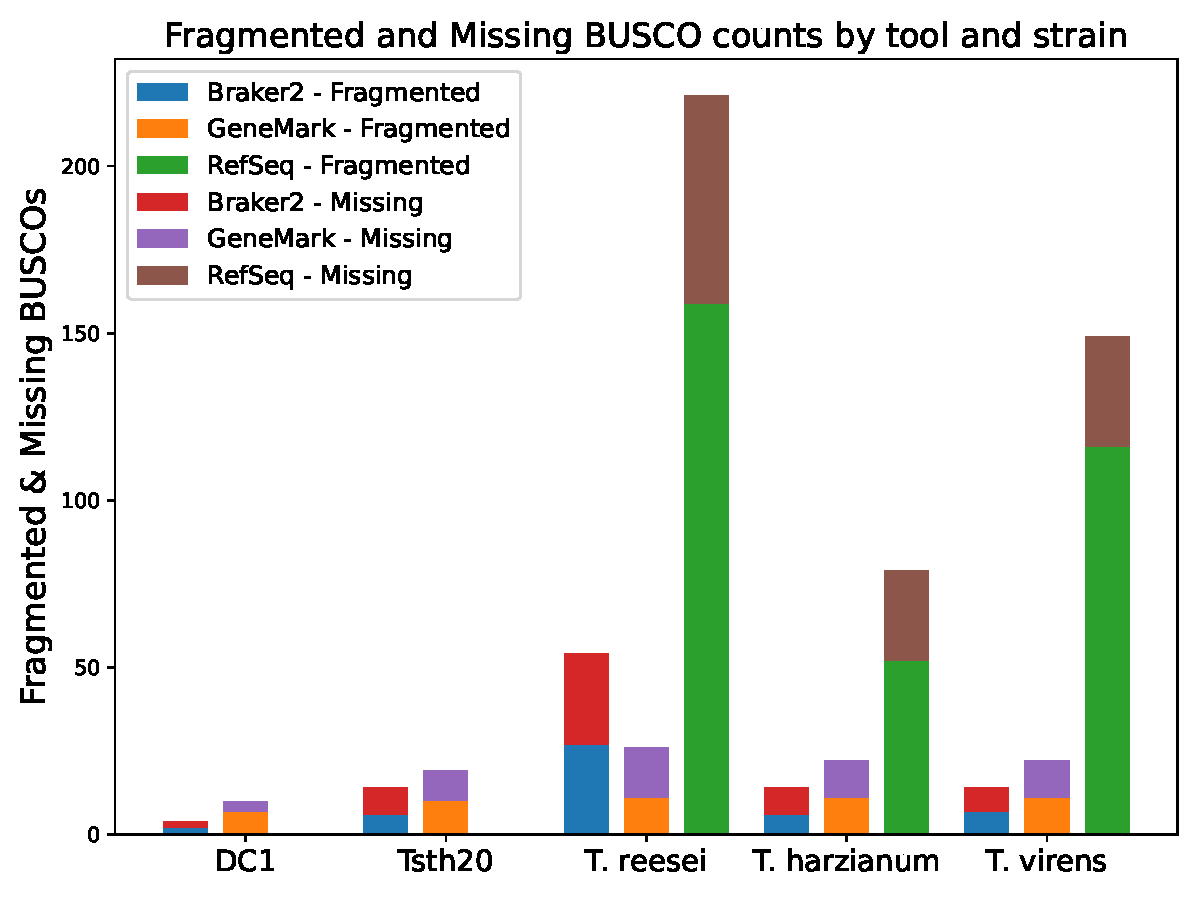
\includegraphics[width=0.90\textwidth]{figures/busco-missing-counts.pdf}
  \caption[Missing BUSCO counts]{Barplot showing the number of missing BUSCOs for each gene finder across all \textit{Trichoderma} genome assemblies. For DC1 and Tsth20, RefSeq annotations are not available, so their values are set to 0. The dashed line indicates the total number of BUSCO markers in the selected dataset (4323).}
  \label{fig:busco-missing}
\end{figure}

\begin{table}
  \begin{center}
    \begin{subtable}{\textwidth}
      \centering
      \begin{tabular}{|c|c|c|c|c|c|c|}
        \hline
        Strain & Complete & Single & Duplicated & Fragmented & Missing \\ \hline
        DC1 & 4319 & 3505 & 814 & 2 & 2 \\ \hline
        Tsth20 & 4309 & 3575 & 734 & 6 & 8 \\ \hline
        \textit{T. reesei} & 4269 & 3616 & 653 & 27 & 27 \\ \hline
        \textit{T. harzianum} & 4309 & 3562 & 747 & 6 & 8 \\ \hline
        \textit{T. virens} & 4309 & 3504 & 805 & 7 & 7 \\ \hline
      \end{tabular}
      \caption{Braker2}
      \vspace{0.5cm}
    \end{subtable}
    \begin{subtable}{\textwidth}
      \centering
      \begin{tabular}{|c|c|c|c|c|c|c|}
        \hline
        Strain & Complete & Single & Duplicated & Fragmented & Missing \\ \hline
        DC1 & 4313 & 4311 & 2 & 7 & 3 \\ \hline
        Tsth20 & 4304 & 4291 & 13 & 10 & 9 \\ \hline
        \textit{T. reesei} & 4297 & 4297 & 0 & 11 & 15 \\ \hline
        \textit{T. harzianum} & 4301 & 4291 & 10 & 11 & 11 \\ \hline
        \textit{T. virens} & 4301 & 4291 & 10 & 11 & 11 \\ \hline
      \end{tabular}
      \caption{GeneMark}
      \vspace{0.5cm}
    \end{subtable}
    \begin{subtable}{\textwidth}
      \centering
      \begin{tabular}{|c|c|c|c|c|c|c|}
        \hline
        Strain & Complete & Single & Duplicated & Fragmented & Missing \\ \hline
        \textit{T. reesei} & 4102 & 4101 & 1 & 159 & 62 \\ \hline
        \textit{T. harzianum} & 4244 & 4234 & 10 & 52 & 27 \\ \hline
        \textit{T. virens} & 4174 & 4164 & 10 & 116 & 33 \\ \hline  
      \end{tabular}
      \caption{RefSeq}
    \end{subtable}
  \end{center}
  \caption{Results from BUSCO using the fungal analysis option
    organized by gene finding tool. The selected BUSCO dataset
    contains 4323 markers. For more information on the categories
    assigned by BUSCO, please refer to the documentation.}
  \label{table:busco}
\end{table}

While BUSCO matches are a good metric for general performance of gene
finders, it is also important to investigate BUSCO proteins without
matching gene predictions. Table \ref{table:busco}, shows breakdowns
of genes missed by each gene finder across the \textit{Trichoderma}
assemblies. 


%\begin{center}
% \begin{table}
% \makebox[\textwidth]{
% \begin{tabular}{|c|c|c|c|c|c|c|c|}
%   \hline
%   Tool & BUSCO ID & Annotation & DC1 & Tsth20 & \textit{T. reesei} & \textit{T. harzianum} & \textit{T. virens} \\ \hline
%   Braker2 & 195619at4751 & \makecell{Pyridoxal phosphate-dependent \\ transferase} & \  & \checkmark & \checkmark & \checkmark & \checkmark \\ \hline
%   Braker2 & 285254at4751 & Aminoacyl-tRNA synthetase & \checkmark & \checkmark & \checkmark &  & \checkmark \\ \hline
%   Braker2 & 348020at4751 & Formyl transferase &  &  & \checkmark &  & \checkmark \\ \hline
%   Braker2 & 497024at4751 & Zinc finger C2H2-type &  & \checkmark & \checkmark & \checkmark & \checkmark \\ \hline
%   GeneMark & 195619at4751 & \makecell{Pyridoxal phosphate-dependent \\ transferase} &  & \checkmark & \checkmark & \checkmark & \checkmark \\ \hline
%   GeneMark & 285254at4751 & Aminoacyl-tRNA synthetase & \checkmark & \checkmark & \checkmark &  & \checkmark \\ \hline
%   GeneMark & 348020at4751 & Formyl transferase &  &  &  &  & \checkmark \\ \hline 
%   GeneMark & 438731at4751 & LSM domain & \checkmark & \checkmark &  & \checkmark & \checkmark  \\ \hline
%   GeneMark & 470813at4751 & Ubiquitin-conjugating enzyme &  &  &  &  &  \\ \hline
%   GeneMark & 497024at4751 & Zinc finger C2H2-type &  & \checkmark & \checkmark & \checkmark & \checkmark \\ \hline
%   RefSeq & 494at4751 & Midasin & N/A & N/A &  &  & \checkmark\\ \hline
%   RefSeq & 315802at4751 & tRNA dimethylallyltransferase & N/A & N/A & \checkmark & \checkmark &  \\ \hline
%   RefSeq & 352224at4751 & YEATS & N/A & N/A &  & \checkmark &  \\ \hline
% \end{tabular}
% }
% \caption[GeneMark missed BUSCO proteins]{The presence (\checkmark)
%   or absence of all BUSCO IDs missed by Braker2, GeneMark and RefSeq
%   in each \textit{Trichoderma} assembly.}
% \label{table:genemark-busco}
%\end{table}
%\end{center}

%\begin{table}
%  \centering
%  \begin{tabular}{|c|c|c|c|c|c|c|}
%    \hline
%    BUSCO ID & Annotation & DC1 & Tsth20 & \textit{T. reesei} & \textit{T. harzianum} & \textit{T. reesei} \\ \hline
%    494at4751 & Midasin & N/A & N/A & X & X & \checkmark\\ \hline
%    315802at4751 & tRNA dimethylallyltransferase & N/A & N/A & \checkmark & \checkmark & X \\ \hline
%    352224at4751 & YEATS & N/A & N/A & X & \checkmark & X \\ \hline
%  \end{tabular}
%  \caption[RefSeq missed BUSCO proteins]{The presence (\checkmark) or
%    absence (X) of all BUSCO IDs missed by RefSeq in each
%    \textit{Trichoderma} assembly.}
%  \label{table:refseq-busco}
%\end{table}

Braker2, GeneMark and RefSeq all demonstrate excellent coverage of the
BUSCO fungal protein set, indicating that these gene finders are
capable of predicting genes that are expected to be present in these
assemblies. From this we can say that the foundations of the
underlying gene models used by each gene finder are solid. Braker2
produces more duplicate matches than GeneMark and RefSeq, but this is
likely due to multiple isoforms of possible genes being present in the
input data. Despite excellent coverage of the BUSCO fungal proteins,
all three gene finders miss some BUSCO proteins in their
predictions. 
Finally, we reiterate the possibility that human curation of RefSeq datasets is responsible for these differences, but this requires further investigation.

\section{Region Identification}
\label{section:regions}

Visual breakdowns of the types of regions identified and their counts
for each \textit{Trichoderma} assembly are shown in figure
\ref{fig:regions-sankey}. We will discuss the types of regions,
beginning with fully supported regions. These regions, labelled `Full
Support', are sections of genomic sequence where each gene finder
agrees that a gene is present in some form. These fully supported
regions are then broken down into two categories, based on whether or
not the models from each gene finder agree on the start and/or stop
positions of the gene model. Regions that have support from more than
one gene finder, but not all, are labelled regions with `Partial
Support'. These regions are also broken down in to two subtypes based
on whether or not the gene predictions agree on the start and/or stop
positions of the gene. Regions with support from only one gene finder
are labelled as singletons.

\begin{figure}
  \centering
  \begin{subfigure}{0.9\textwidth}
    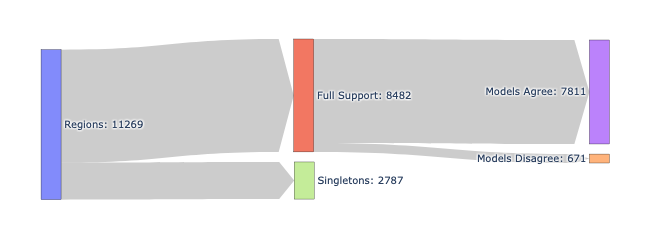
\includegraphics[width=\textwidth]{figures/dc1-region-breakdown.png}
    \label{fig:dc1-regions}
    \caption{DC1}
  \end{subfigure}
  \begin{subfigure}{0.9\textwidth}
    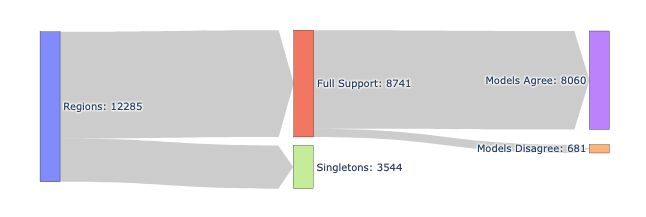
\includegraphics[width=\textwidth]{figures/tsth20-region-breakdown.png}
    \label{fig:tsth20-regions}
    \caption{Tsth20}
  \end{subfigure}
  \begin{subfigure}{0.9\textwidth}
    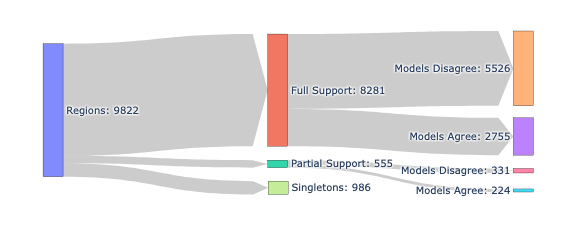
\includegraphics[width=\textwidth]{figures/t-reesei-region-breakdown.png}
    \label{fig:t-reesei-regions}
    \caption{\textit{T. reesei}}
  \end{subfigure}
\end{figure}
\begin{figure}
  \ContinuedFloat
  \centering
  \begin{subfigure}{0.9\textwidth}
    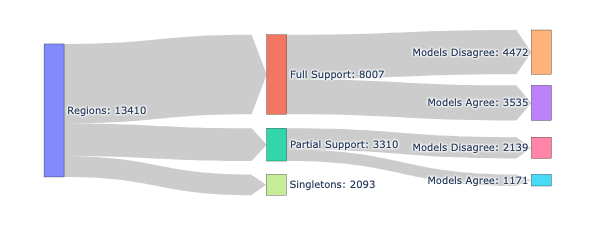
\includegraphics[width=\textwidth]{figures/t-harzianum-region-breakdown.png}
    \label{fig:t-harzianum-regions}
    \caption{\textit{T. harzianum}}
  \end{subfigure}
  \begin{subfigure}{0.9\textwidth}
    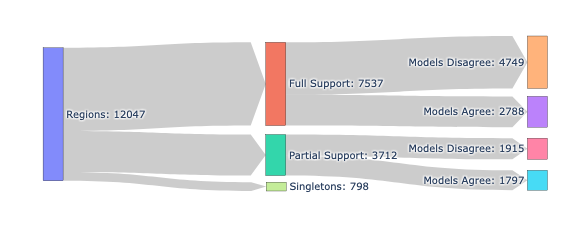
\includegraphics[width=\textwidth]{figures/t-virens-region-breakdown.png}
    \label{fig:t-virens-regions}
    \caption{\textit{T. virens}}
  \end{subfigure}
  \caption[Breakdown of identified regions]{Figures showing breakdowns
    of genomic regions identified by the region finding
    process. Regions, in blue, are categorized based on support from
    gene finders. Regions with supporting predictions from all gene
    finders included in this analysis are labelled with `Full Support'
    and colored red. Fully supported regions are then broken down into
    regions where gene models agree on the start and stop positions of
    the genes (purple), and those that do not (orange). Regions
    labelled with `Partial Support' (turquoise) are regions with
    supporting gene predictions from more than one gene finder, but
    not all. Partially supported regions are also broken down into
    regions in which gene finders agree on the start and stop
    positions of the gene (cyan), and those that do not agree
    (pink). Regions with gene predictions from only one gene finder
    are labelled as singletons (green).}
  \label{fig:regions-sankey}
\end{figure}

Looking at DC1 and Tsth20 in figure \ref{fig:regions-sankey}, it
appears that Braker2 and GeneMark predict genes in the same regions in
the majority of cases. For regions with full support, the models also
tend to agree on the start and stop positions of the gene in that
region. This is not generally the case as we will see later. There are
no regions with partial support for DC1 and Tsth20, as there are only
two gene finders considered, leaving only complete agreement or
disagreement. \textit{Trichoderma reesei} contains the fewest number
of regions, which seems to scale appropriately with the total number
of predicted genes and assembly length. The vast majority of the
regions are fully or partially supported by Braker2, GeneMark and
RefSeq, with only 10 percent of the regions being single
predictions. The most interesting observation here is the number of
fully supported regions that disagree on start and stop positions of
the gene(s) in each region. There is clearly a difference in the gene
models being produced by these gene finders. If there is also more
disagreement on the start and stop positions of a gene, then there is
likely disagreement on the number and location of exons and introns
within the gene model as well. In the case of partially supported
regions, there is more disagreement than agreement, but that may come
as less of a surprise as there is already disgreement on presence by
definition. Gene finding behaviour in regions from
\textit{T.harzianum} and \textit{T. virens} differ from the other
assemblies in the split between fully and partially supported
regions. There seems to be fewer regions with full support from all
gene finders and the reason why is unclear. The gene models in each
region, whether fully or partially supported, still tend to disagree
on start and stop positions of the genes more often than agree.

It is also worthwhile investigating some potentially interesting cases
of strange gene calls in regions. One such case is when a region
contains more than three individual predicted genes. The null
hypothesis, so to speak, is that if all gene finders agree exactly on
the presence and position of a gene in a region, then one should
expect exactly three predictions in that region. We observe that this
is not always true. Cases of more than three gene predictions in a
region were present in regions from all processed assemblies. Figure
\ref{fig:uncertain-regions} shows an example of one of these regions,
in which the single gene predicted by RefSeq spans multiple gene
predictions from both Braker2 and GeneMark. In the case of DC1 and
Tsth20, there were very few regions that matched this scenario, with
19 and 6 regions matching, respectively. Conversly, \textit{T. reesei,
  T.harzianum and T.virens} contain many such regions, with assemblies
reporting 546, 899 and 521 regions with greater than three gene
predictions, respectively. While having predictions from each gene
finding tool present in a region is a strong indicator for the
presence of a gene, having more than one gene prediction per gene
finder raises questions about which model (or models) is correct and
why disagreement exists.

\begin{figure}
  \centering
  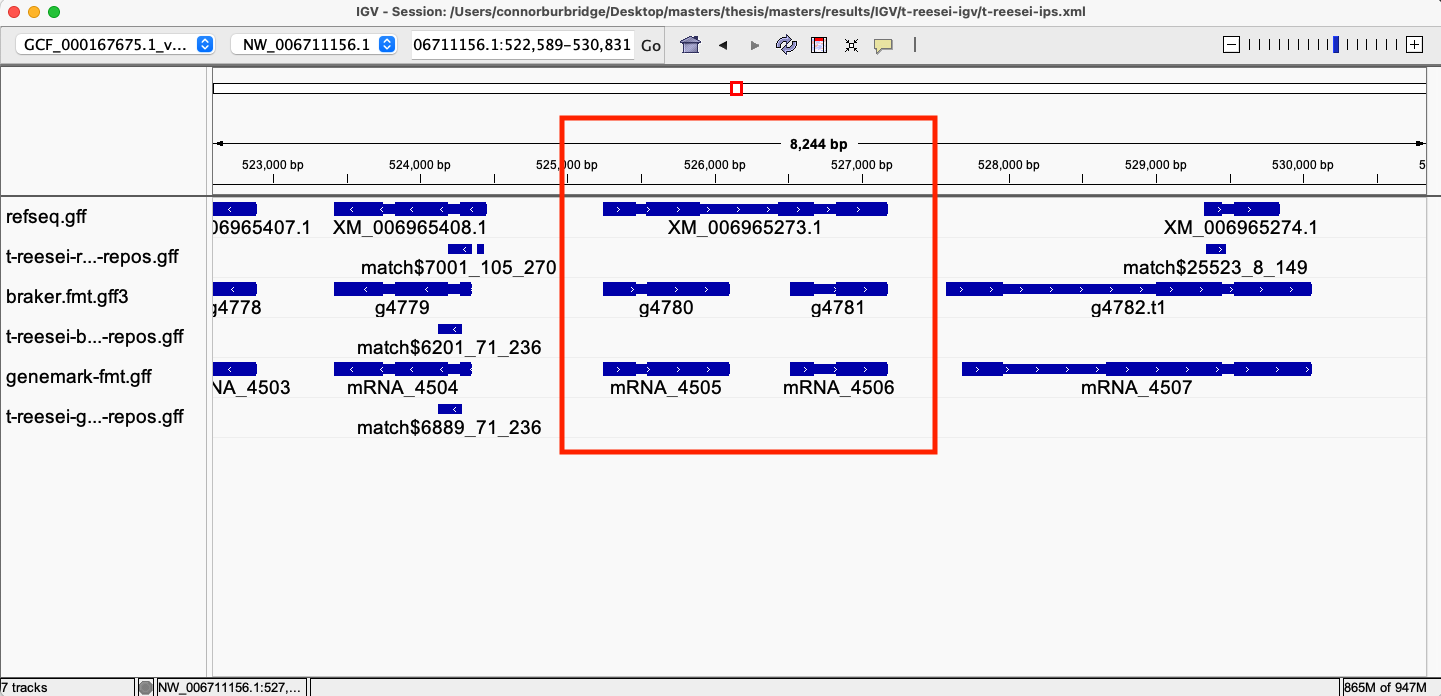
\includegraphics[width=0.9\textwidth]{figures/igv/igv-uncertain-regions.png}
  \caption[Example of a region with many gene calls]{An IGV screenshot
    from \textit{T. reesei} showing a region containing five
    gene predictions.}
  \label{fig:uncertain-regions}
\end{figure}

Another interesting set of criteria to investigate is whether or not
gene finders always predict genes on the same strand within a
region. We observe that regions containing predictions on different
strands do exist, and are observed in predictions from all assemblies
included in this analysis. Figure \ref{fig:opposing-strands} shows an
example of a region containing gene predictions on opposing
strands. As in the case of regions with more than three gene
predictions, DC1 and Tsth20 report fewer mixed strand regions with DC1
reporting 29 regions and Tsth20 reporting 46. \textit{T. reesei,
  T. harzianum and T. virens} report more regions in which this
property is true, with region counts being 203, 533 and 293
respectively. Under the assumption that gene finders should predict
the same genes on the same strands, it is unexpected to find so many
of these cases, and will require further investigation.

\begin{figure}
  \centering
  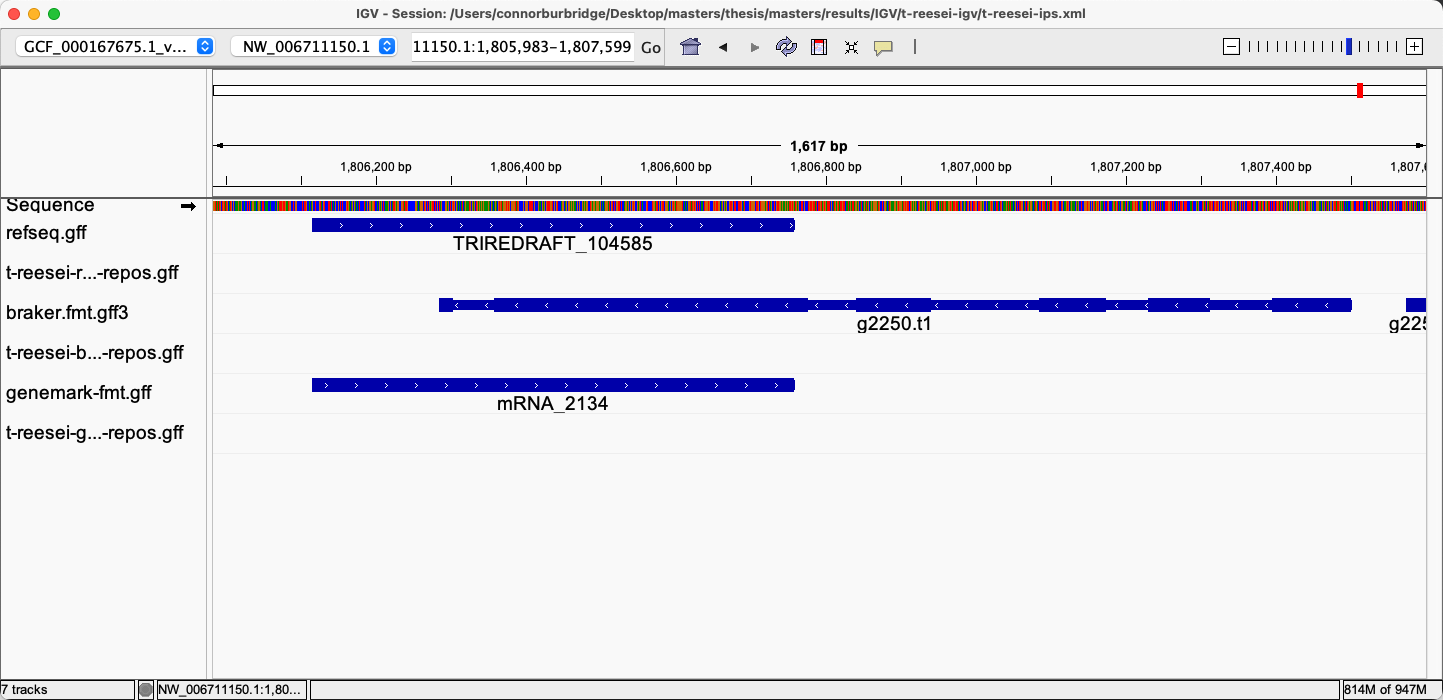
\includegraphics[width=0.9\textwidth]{figures/igv/igv-opposing-strands.png}
  \caption[Predictions on opposing strands]{An IGV screenshot of
    \textit{T. reesei} showing a region which contains gene
    predictions on opposite strands.}
  \label{fig:opposing-strands}
\end{figure}

In summary, gene finders agree partially or completely on the presence
of a gene in the vast majority of cases. While gene finders generally
agree on the presence of a gene, they tend to disagree on the
underlying gene model more often than they agree, except in in the
case of DC1 and Tsth20. This is likely due to only including two gene
finders in their analysis rather than three, resulting in fewer
opportunities for disagreement. This observation is true when applied
to the start and stop positions of the gene, but further investigation
and comparison of intronic and exonic sequences between genes may
provide more insight. Finally, regions identified in this analysis do
not always fit the ideal scenario of one gene prediction from each
tool per region. Regions in which there are more than three gene
predictions were observed in all assemblies included in this work. In
addition, gene finders do not always predict genes on the same strand
as other gene finders.


\chapter{Conclusions}



%\section{Selection of Gene Finding Tool}
\label{chapter:conclusion}

With all of these results, it makes sense to explore the question of
which gene finding tool one should choose for optimal gene prediction
performance. Comparisons drawn in this section are made in the context
of \textit{Trichoderma} assemblies and may not extend to other
datasets. Observations from the results portion of this work have been
converted to scores relative to the other gene finders. Scores range
from zero to three, with values being: 0 - failing performance, 1 -
passing performance, 2 - good performance, and 3 - excellent
performance. Results from this work are summarized in Table
\ref{table:final-score}. Ignoring availability and use of the gene
finding tools, it would appear that RefSeq performs the best in the
remaining categories, earning top marks in every category except in
it's ability to predict very short genes. Braker2 earns second place;
however, this does not capture Braker2's failure in predicting
accurate numbers of genes in DC1, Tsth20, \textit{T. harzianum} and
\textit{T. virens}. GeneMark comes in last, excelling only in number
of genes predicted and Pfam support for the genes that it predicts.

Relating these observations to use-case scenarios, in the case that
your organism of interest has a RefSeq annotation associated with it,
the RefSeq gene prediction process appears to produce the best set of
predictions. If users also have experimental evidence, such as RNAseq
data under experimental conditions, it may be worthwhile training a
Braker2 model and predicting genes with Braker2 to supplement the
already well performing RefSeq gene predictions. In a similar case, if
the organism is of RefSeq status, but the assembly in question is
novel to the work being performed, training and prediction using a
Braker2 model with experimental evidence either from the novel genome
or from the RefSeq accession in addition to use of the RefSeq
annotation would likely be the best option. If the organism of
interest is not a RefSeq individual but training data is available for
that organism, Braker2 is the next best option, although it is
important to note that the application of a trained Braker2 prediction
model to an organism from which the training data did not originate is
not advised based on the results presented in this work (see
\ref{section:gene-finding}). While it is true that the
\textit{T. reesei} genome differs from other \textit{Trichoderma}
genomes, it's status as a representative RefSeq organism makes it
somewhat of a gold standard. In this case, applying a gene model
trained using evidence from the gold standard produces biased numbers
of genes predicted in other \textit{Trichoderma} genomes. While
Braker2 technically scores the second highest, users must be very
careful when selecting training data, and ensure that the training
data either comes from the organism of interest, or comes from a very
closely related organism with a highly similar genome. In the case
that no appropriate training data is available, GeneMark is still an
option, and users can be confident that the tool predicts a reasonably
accurate number of genes with supporting Pfam matches. It is also
important to note that GeneMark does not perform as well in AT-rich
regions as Braker2 and RefSeq, does not predict isoforms, and
systematically fails to predict some BUSCO orthologs.

When availability of a gene finding tool becomes a concern and RefSeq
is not considered, the scores drop significantly for Braker2 and
GeneMark as seen in the final row of Table \ref{table:final-score}. In
this situation, Braker2 still outperforms GeneMark. If the organism of
interest is not considered a representative RefSeq individual, but
supporting evidence specific to that organism or a very closely
related organism is available, a trained Braker2 prediction model will
perform well. Again, in the case that the organism is not a RefSeq
individual and no appropriate training data is available, GeneMark is
still a reasonable option even with the previously identified caveats.

\begin{table}
  \centering
  \begin{tabular}{|c|c|c|c|}
    \hline
    Category & Braker2 & GeneMark & RefSeq \\ \hline
    Availability & 3 & 3 & 0 \\ \hline
    Ease of install & 1 & 2 & 0 \\ \hline
    Ease of use & 3 & 3 & 0 \\ \hdashline
    \makecell{\# of genes\\predicted} & 0 & 3 & 3 \\ \hline
    \makecell{\# of transcripts\\predicted} & 3 & 0 & 2 \\ \hline
    \makecell{Predicts shortest\\genes} & 2 & 1 & 0 \\ \hline
    \makecell{Predicts more\\shorter genes} & 1 & 0 & 3 \\ \hline
    BUSCO Performance & 2 & 1 & 3 \\ \hline
    \makecell{Performance in\\AT-rich sequence} & 2 & 1 & 3 \\ \hline
    \makecell{Predictions with \\InterProScan support} & 3 & 3 & 3 \\ \hline
    \makecell{Final Score\\(Publicly Available)} & 20 & 17 & N/A \\ \hline
    \makecell{Final Score\\(Ignoring Availability)} & 13 & 9 & 17 \\ \hline
  \end{tabular}
  \caption[Final scoring table]{Table with scores attributed to
    performance of each gene finder in several categories. The score
    definitions for performance are as follows: 0 - fail, 1 - pass, 2
    - good, 3 - excellent. Since RefSeq is not publicly available, it is
    marked as N/A in the publicly available final scores. The dashed
    line separates categories associated with availability and use
    from categories describing gene prediction performance.}
  \label{table:final-score}
\end{table}

In summary, these results indicate that if your organism is a RefSeq
organism, use the RefSeq annotation. If no RefSeq predictions are
available but appropriate training data is, one should use Braker2. If
the training data is of questionable similarity or not available at
all, users can fall back on \textit{ab initio} gene finders such as
GeneMark, which while not ideal, still predict genes with supporting
evidence.

\section{Future Work}

While this work is extensive, there are still many areas that could be expanded on. The sheer number of gene finding tools available means that many more could be compared to the ones presented here. In addition, supplying more training data to Braker2 may improve gene finding performance, and training on RNAseq from different organisms could be used to improve the performance of Braker2. It is clear from the results that Braker2 performed worse than GeneMark and the RefSeq predictions, which was likely due to the training data being used from \textit{T. reesei}. Different types of training data such as RNAseq, expressed sequence tags (ESTs), and protein sequences could also be used to train models that support external evidence. Another limitation of this work is that the gene finders were run with default parameters, and it is possible that tuning the parameters of the gene finders could improve performance.

Following the gene prediction process, there are a number of different analyses that could be performed on the predicted genes. For example, functional annotation of the predicted genes could be performed using tools such as BLAST2GO to assign Gene Ontology (GO) terms and KEGG pathways to the predicted genes. This could provide further insight into the functional roles of the predicted genes and their potential applications. More importantly in the context of this work, analysis of predicted genes with a tool like antiSMASH could be used to identify biosynthetic gene clusters (BGCs) in the predicted genes. 

Expanding the number of genomes used in this work would also be beneficial, as the results presented here are based on a limited number of genomes. Including more genomes from different species and strains of \textit{Trichoderma} could provide a more comprehensive understanding of gene finding performance across the genus. Additionally, comparing the performance of gene finders on other fungal genomes could provide insights into whether the findings are generalizable. Examining the performance of gene finders on different assemblies of the same genome could also be useful, as different assemblies may have different levels of completeness and accuracy. This could help to identify tangible benefits of using one assembly over another, and could also provide insights into the limitations of gene finders when applied to different assemblies.

Finally, the results of this work could be used to inform future research in the field of fungal genomics, particularly in the case of the DC1 and Tsth20 genome assemblies. The results of these genome assemblies are high-quality, and contain near-chromosomal scale sequences. The predicted genes from these genomes are a rich resource for future research, and could be used to identify novel genes and gene families in DC1 and Tsth20. Further understanding of the mechanisms behind salt and drought tolerance as well as degradation of hydrocarbon in sub-optimal environments could be achieved by studying the predicted genes in these genomes. 


%\chapter{Discussion}
%\section{Assemblies of DC1 and Tsth20}
Overall, the assemblies of DC1 and Tsth20 resulted in what can be
described as sequences suitable for further downstream
processing. Assembled lengths for both samples are similar to closely
related \textit{Trichoderma} accessions, indicating that the
assemblies are of appropriate length, but this could be confirmed with
further wetlab experiments in the future. The assembly of DC1 resulted
in eight contigs, with two sequences, ctg000040 being significantly
shorter at 65Kb than it's counterparts, which deviates from the
expected 7 chromosome-scale contigs expected from a
\textit{Trichoderma} assembly\cite{Kubicek2019}. Why this sequence is
significantly shorter than other contigs is unclear, but could arise
for several reasons. The most obvious reason would be mis-assembly,
which could arise from complications caused by both the anomolous GC
content reginos as well as highly repetitive regions. Even with the
inclusion of Nanopore sequencing data, it is possible that there was
insufficient support for connection between these contigs and
others. This highlights the complexity of assembling sequences with
anomolous content and supports the idea that multiple rounds and forms
of sequencing data may be required to produce scaffold and reference
level assemblies of non-model organisms. Another possible explanation
for an unaccounted for contig could be the assembly of a mitochondrial
genome, although this appears somewhat unlikely due to the length of
the ctg000040, it is not entirely out of the question. Previous work
focusing on mitochondrial genomes in \textit{Trichoderma} shows the
lengths of mitochondrial assemblies from six \textit{Trichoderma}
samples to be between 27Kb and 42Kb.

The assembly of Tsth20 resulted in seven contigs, matching that of the
expected seven chromosomes detected in most \textit{Trichoderma}
strains. The total assembled length of Tsth20 is again similar but
slightly larger than existing \textit{Trichoderma} assemblies.

%\section{Initial Gene Counts}
Initial gene counts from Braker2 and Genemark show a similar trend in
all assemblies included in this analysis. Braker tends to predict
fewer genes in comparison to GeneMark and RefSeq results except in the
case of \textit{T. reesei}. The cause of this difference is likely
two-fold in nature. Most importantly, Braker2 was trained on an RNAseq
dataset derived from \textit{T. reesei}. This additional information
in the gene finding model is likely why Braker2 finds more genes and
transcripts than GeneMark. The effects of this training set may also
be why Braker2 tends to predict fewer genes and transcripts in other
assemblies when compared to results from GeneMark and RefSeq. The
nature of gene models in \textit{T. reesei} likely differs than those
of other genomes, resulting in 'poorer' relative performance than in
\textit{T. reesei}. This highlights the fact that users should choose
training sets carefully when planning to use a hybrid gene finding
approach. Choosing a dataset that is inappropriate will end with
results that are skewed or biased towards the training set of
interest, although they will likely be of higher confidence. This is
an important trade-off to consider when preparing for a hybrid gene
finding approach.

Another potential explanation of Braker2's low gene count trend could
again be due to the reference training set used in training. However
in this case, not necessarily due to the RNAseq data itself, but the
nature and size of the genome from whih the RNAseq data was gathered
from. The \textit{T. reesei} genome is significantly smaller than
other assemblies considered as shown in figure (blah), resulting in
less physical space for coding sequences to be found. This would
explain why GeneMark predicts a similar number of genes as Braker2 in
\textit{T. reesei} but not in any of the other assemblies. In theory,
it would make sense that after training, Braker2 would predict a
fraction of all possible genes in a larger assembly, since it was
trained with RNAseq data from a genome that is a fraction of the
size. Again, this shows that the choice of training data is paramount
when planning a hybrid assembly approach to gene finding.



%\section{BUSCO Analysis}

The results from BUSCO analysis of the gene sets produced by each
prediction method prove promising. With all gene sets being 99.2\%
complete or higher based on the fungal dataset provided to BUSCO. This
higher number indicates that these gene finding tools capture nearly
completely the set of evolutionarily conserved single-copy orthologs
pre-defined by BUSCO curators. In the case of the fungal dataset,
there are 758 genes considered during analysis.

The most glaring observation from this analysis is the duplication
level found in the gene sets produced by Braker2 in comparison to the
GeneMark and RefSeq datasets. The Braker gene sets show a single-copy
match for roughly 80-85\% of the total gene call set with duplicates
making up the other 15-20\% of the set. The likliest reason for this
difference is the presence of isoforms in gene sets produced by
Braker. As shown in figure \ref{fig:genecounts}, Braker2 does produce
isoforms in it's output, which would be identified as duplicates in
the BUSCO process. However, the number of isoforms predicted per gene
does not make up 20\% of the total set of gene calls. It is possible
that the BUSCO dataset contains a large fraction of the Braker2 gene
calls with isoforms, but that is unlikely and warrants further
investigation into the genes matching the BUSCO dataset.  Another
possible explanation is that Braker2 is predicting genes that are
actually isoforms as separate genes. BUSCO also makes note of isoforms
of a gene being the cause of high number of duplicates, and recommends
users remove isoforms prior to running BUSCO, although that step was
not performed for this work.






\uofsbibliography{./refs/full-bib}

%\chapter{Supplemental Information}
\section{Platform and Software Installation}
(Possibly supporting materials or discussion)

\subsection{Platform}
All analysis was performed on the RSMI server hosted on Copercius at
the University of Saskatchewan. This server is equipped with 64 cores
in addition to 1.5 TB of memory. The server is running RedHat
Enterprise Linux 7 as of writing this thesis. All data is stored
either on datastore, or in the RSMI scratch space.

\subsection{NextDenovo and NextPolish Installation}
Installation of nextDenovo was straightforward. Simply download the
compressed tar file from their website and unpack it. NextDenovo
requires Python versions 2 and 3 along with a package called parallel
to aid in parallel processing of datasets. The parallel package was
installed using pip in the bioinformatics conda environment in the
scratch space of Copernicus. NextPolish was installed in a Python
environment by a member of the research computing team that manages of
our system. Assistance was required for this as the version of RHEL
used by the server introduces glibc version conflicts with Anaconda
when trying to install nextPolish. 

\subsection{RepeatMasker Installation}

The installation procedure was somewhat indepth, requiring
RepeatMasker configuration, which itself requires downloading an
appropriate repeat database (Dfam in this case, included with
RepeatMasker), installation of Tandem Repeat Finder (TRFM) and
installation of a sequence search tool, for which I chose HMMER from
the list of potential tools as we were generally familiar with its
use. The path to the installation of TRFM is required during
configuration along with the search tool of choice, a simple selection
of 4 tools that will have an autocompleted path in this case, since
HMMER is installed via anaconda.

\subsection{GeneMark-ES Installation}
GeneMark-ES was successfully installed by downloading and unpacking
the package from their website along with a key required for use.

\subsection{Braker2 Installation}
Braker2 was also successfully installed by a member of the research
computing team who has set up several modules including an
initialization script to get things up and running as well as create a
reloadable environment for use again in the future. Once the
environment has been loaded, one must load the Hisat2 module from
Compute Canada as well as an htslib module (more detail to come). Once
all modules are loaded, there are a few environemnt variables that
need to be set, those being AUGUSTUS\_CONFIG\_PATH and
TSERBA\_CONFIG(?figure this out). In addition, a software package named
TSEBRA from the same developers as Braker2 must be installed for
consolidating gene calls. The variables can be set within the
braker2.pl command, which have higher priority over environment
variables and probably makes things easier to track.



\end{document}
